% -----------------------------------------
% Classe do documento ufabcFHZh.cls
% -----------------------------------------
% ----------------------------------------- Versão final em português
\documentclass[dsc, EN]{ufabcFHZh}
% -----------------------------------------

% ========== Novos comandos para escrever nomes pré-formatados
%% =============================
%%      IMPORTANTE
%% ESTE ARQUIVO DEVE ESTAR SALVO COMO
%%      UTF - 8
%% =============================

% ----------------------------------------------------------
% Este capítulo é parte integrante do arquivo mestre
% Relatorio_TCC_Mestrado_Base_VERSÃO_SUBVERSÃO
% ----------------------------------------------------------

%==== Novos comandos para escrever nomes pré-formatados
%---
\newcommand{\ufabcFHZ}
{\textbf{\textit{ufabcFHZh.cls}}}
%---
\newcommand{\abntFHZ}
{\textbf{\textit{abntFHZ5.bst}}}
%---
\newcommand{\Fonte}[1]
{{\footnotesize Fonte: #1.}}
%---
\newcommand{\Oautor}
{O autor}
%---
\newcommand{\matlab}
%{Matlab$^\circledR$}
{Matlab\textsuperscript{\textregistered}}
%---
\newcommand{\simulink}
{Simulink\textsuperscript{\textregistered}}
%---
\newcommand{\matlabsimulink}
{Matlab/Simulink\textsuperscript{\textregistered}}
%---
\newcommand{\arduino}
{Arduino\textsuperscript{\textregistered}}
%---
\newcommand{\arduinomega}
{Arduino\textsuperscript{\textregistered} Mega}

%---
\newcommand{\DINAMA}
{\textit{DINAMA}}
%---
\newcommand{\excel}
{Excel\textsuperscript{\textregistered}}
%---
\newcommand{\projetoDaniel}
{\textit{Projeto Daniel}}
%---
\newcommand{\notimpossiblenow}
{\textit{Not Impossible\textsuperscript{Now}}}
%---
\newcommand{\caltech}
{\textit{Caltech}}
%====

% ----------------------------------------- 
% Formas de uso de condicional ifthenelse / toogle para selecionar cores de links
% -----------------------------------------
% http://alvinalexander.com/blog/post/latex/two-simple-examples-using-latex-ifthen-package
% http://tex.stackexchange.com/questions/5894/latex-conditional-expression
% -----------------------------------------
\usepackage{etoolbox} 		% Permite o uso de \newtoggle para criar desvios de fluxo
\usepackage{pdfpages}
%---
\newtoggle{LinksComCores} 	% Opção para selecionar entre links sem cores ou coloridos
% ===
% -----------------------------------------

% ----------------------------------------------------------
% Fim Arquivo
% \usepackage[alf, abnt-emphasize=bf, abnt-thesis-year=both, abnt-repeated-author-omit=no, abnt-last-names=abnt, abnt-etal-cite=3, abnt-etal-list=3, abnt-etal-text=it, abnt-and-type=e, abnt-doi=doi, abnt-url-package=none, abnt-verbatim-entry=no]{abntex2cite}

% Set same dot spacing for list of figures/tables and list of symbols 
%\usepackage{tocbasic}

%\newcommand\Dotfill{\cftdotfill{\cftsecdotsep}}
%   \renewcommand{\cftchapleader}{\cftdotfill{\cftsecdotsep}}


\newcommand{\plotdrs}[4]{ 
\begin{figure}[t]
    \centering
    \begin{subfigure}{0.32\textwidth}
        \centering
        % include second image
        \includegraphics[width=\linewidth]{Figuras/drs/#1/doe_200/drs_#2_all_#3_surface.pdf}  
        \caption{Small dataset.}
        \label{fig:drs_#2_#3_200}
    \end{subfigure}
    \begin{subfigure}{0.32\textwidth}
        \centering
        % include second image
        \includegraphics[width=\linewidth]{Figuras/drs/#1/doe_500/drs_#2_all_#3_surface.pdf}  
        \caption{Medium dataset.}
        \label{fig:drs_#2_#3_500}
    \end{subfigure}
    \begin{subfigure}{0.32\textwidth}
        \centering
        \includegraphics[width=\linewidth]{Figuras/drs/#1/doe_1000/drs_#2_all_#3_surface.pdf}  
        \caption{Large dataset}
        \label{fig:drs_#2_#3_1000}
    \end{subfigure}
    \caption{#4}
    \label{fig:drs_#2_#3}
\end{figure}
}

\newcommand{\plothpoboxplot}[3]{ 
\begin{figure}[t]
    \centering
    \begin{subfigure}{0.3\textwidth}
        \centering
        % include second image
        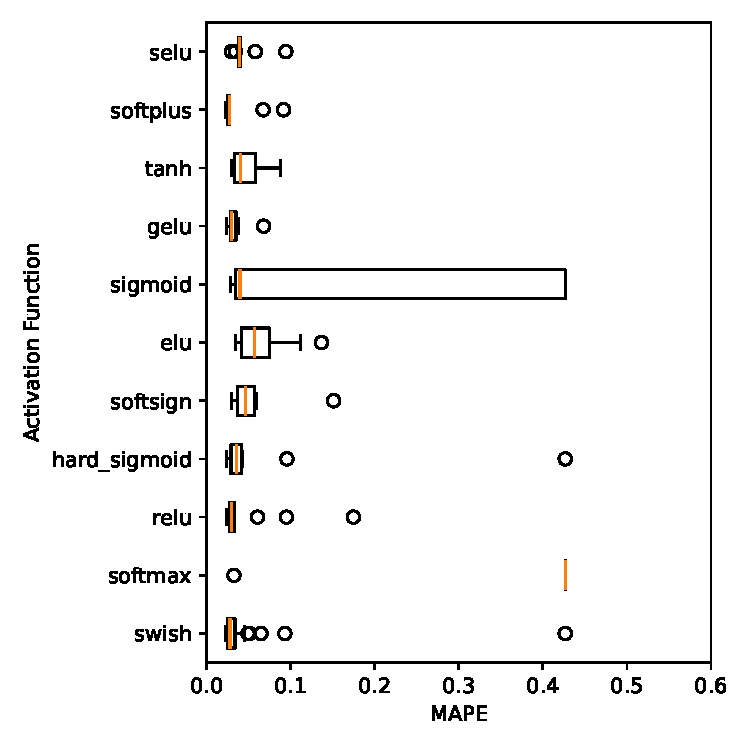
\includegraphics[width=\linewidth]{Figuras/hpo/hpo_plots_#1_#2/hpo_nn_activation_MAPE.pdf}  
        \caption{MAPE.}
        \label{fig:hpo_MAPE_a#1_#2}
    \end{subfigure}
    \begin{subfigure}{0.3\textwidth}
        \centering
        % include second image
        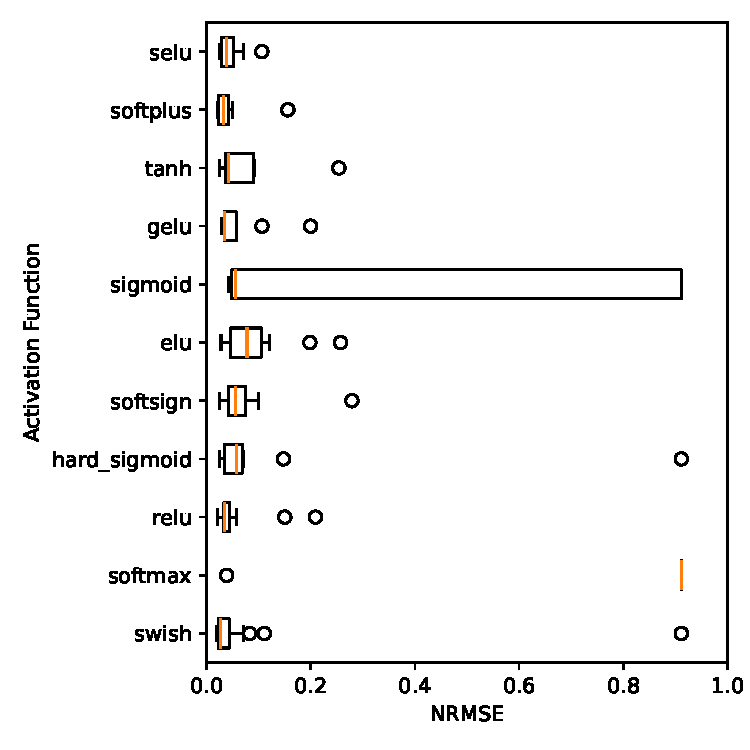
\includegraphics[width=\linewidth]{Figuras/hpo/hpo_plots_#1_#2/hpo_nn_activation_NRMSE.pdf}  
        \caption{NRMSE.}
        \label{fig:hpo_NRMSE_#1_#2}
    \end{subfigure}
    \begin{subfigure}{0.3\textwidth}
        \centering
        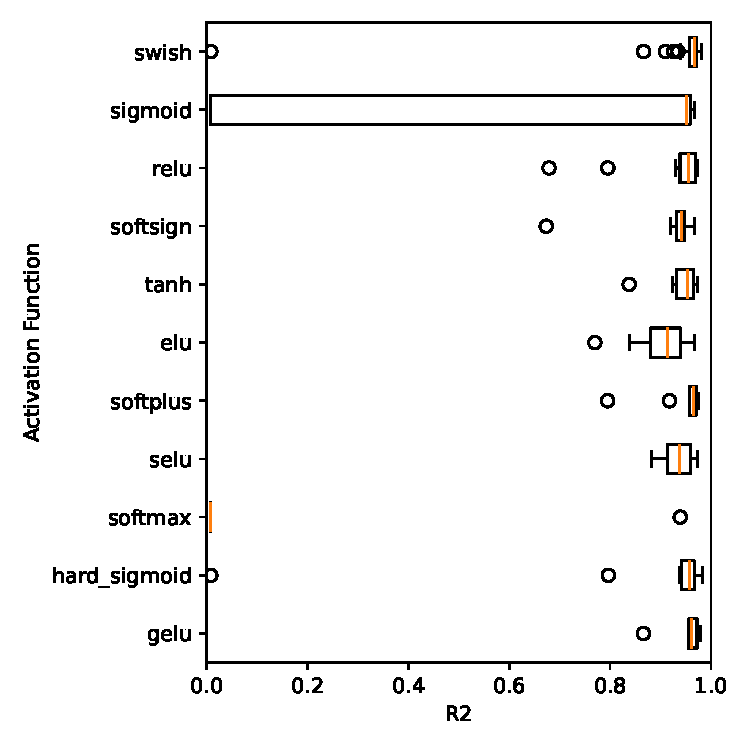
\includegraphics[width=\linewidth]{Figuras/hpo/hpo_plots_#1_#2/hpo_nn_activation_R2.pdf}  
        \caption{R2}
        \label{fig:hpo_R2_#1_#2}
    \end{subfigure}
    \caption{#3}
    \label{fig:hpo_#1_#2}
\end{figure}
}

\newcommand{\plothpomap}[3]{
\begin{figure}[t]
    \centering
    \begin{subfigure}{0.3\textwidth}
        \centering
        % include second image
        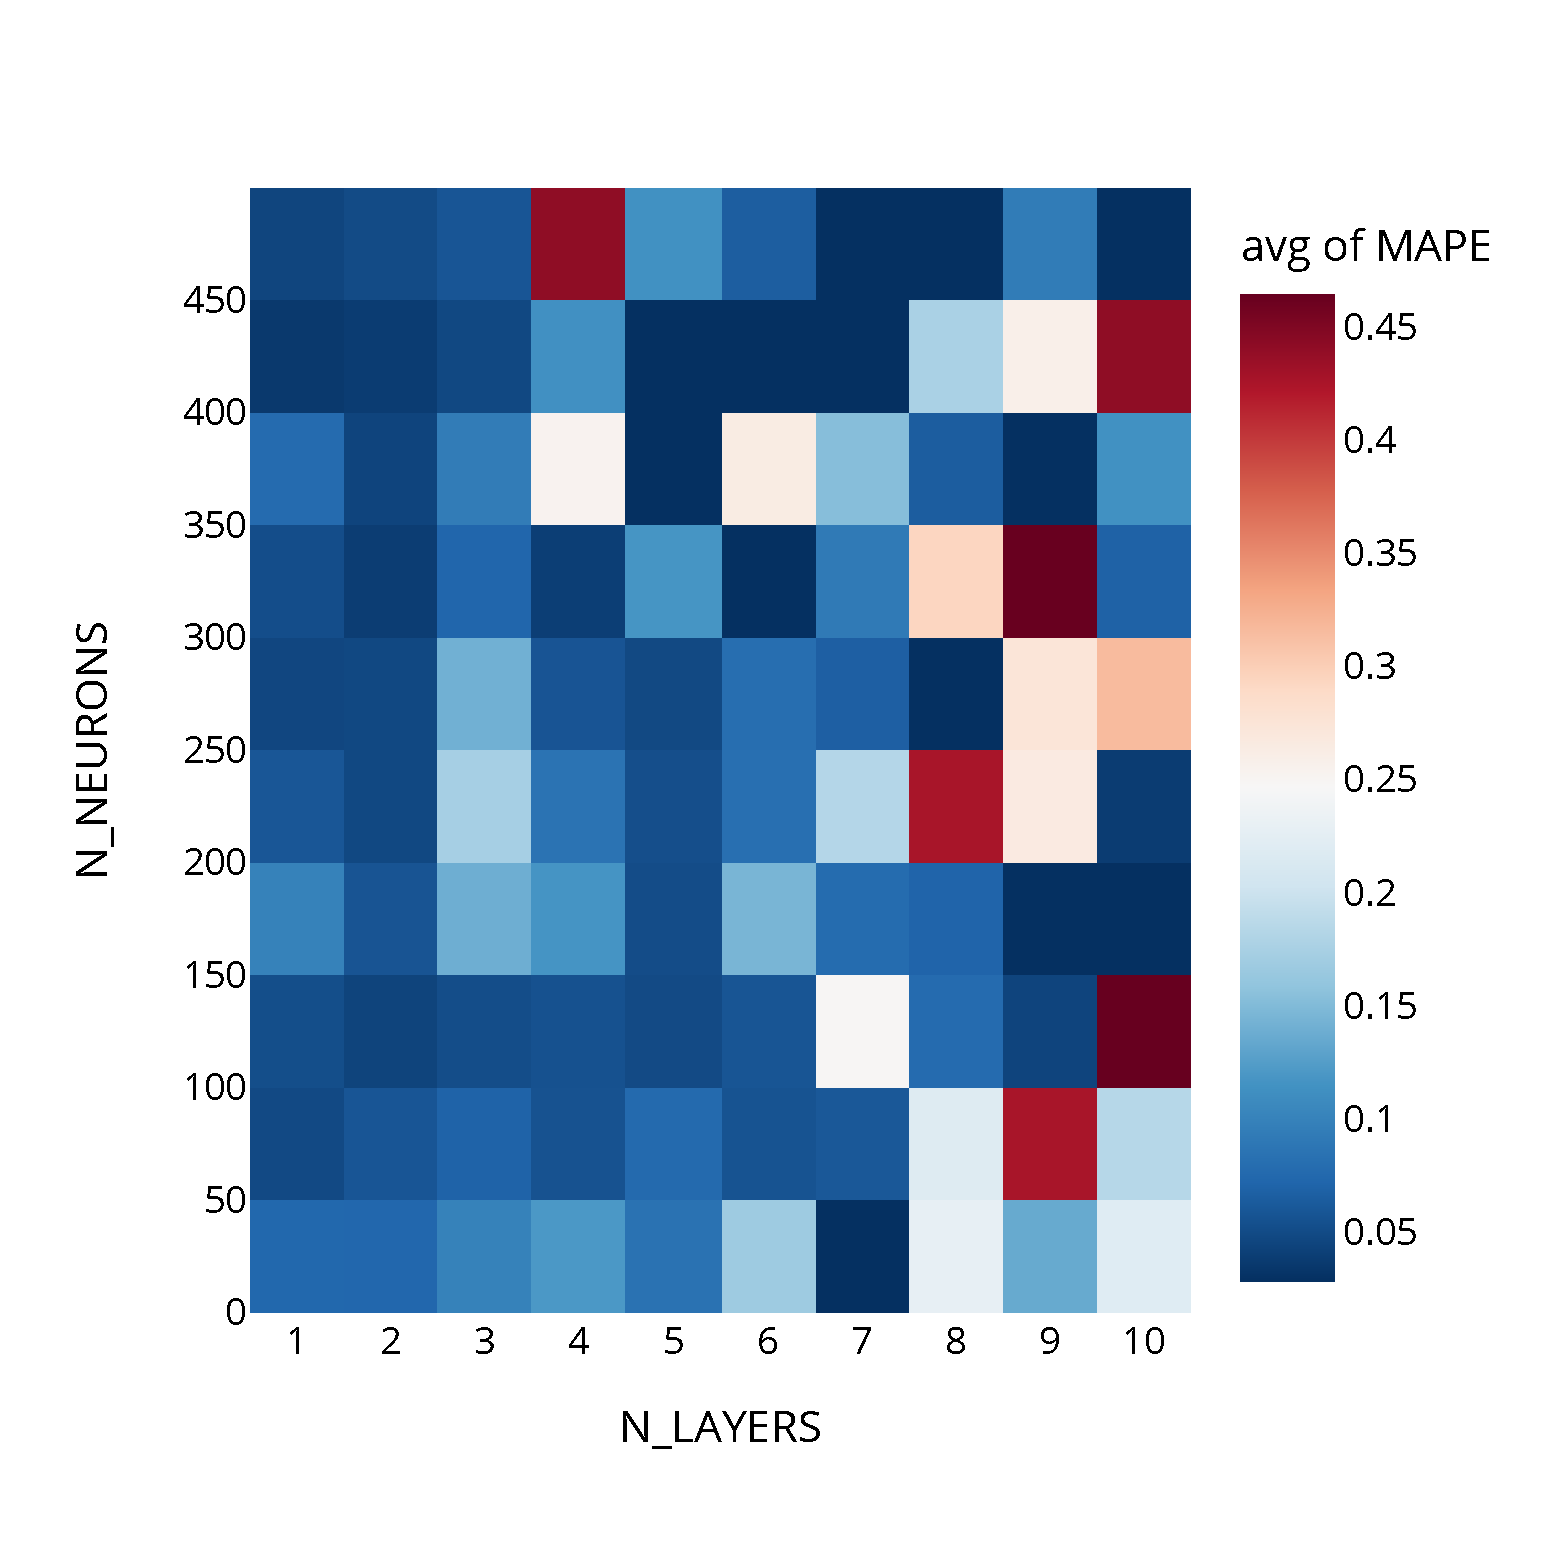
\includegraphics[width=\linewidth]{Figuras/hpo/hpo_plots_#1_#2/neurons_layers_heat_map_MAPE.pdf}  
        \caption{MAPE.}
        \label{fig:hpo_map_MAPE_all_all}
    \end{subfigure}
    \begin{subfigure}{0.3\textwidth}
        \centering
        % include second image
        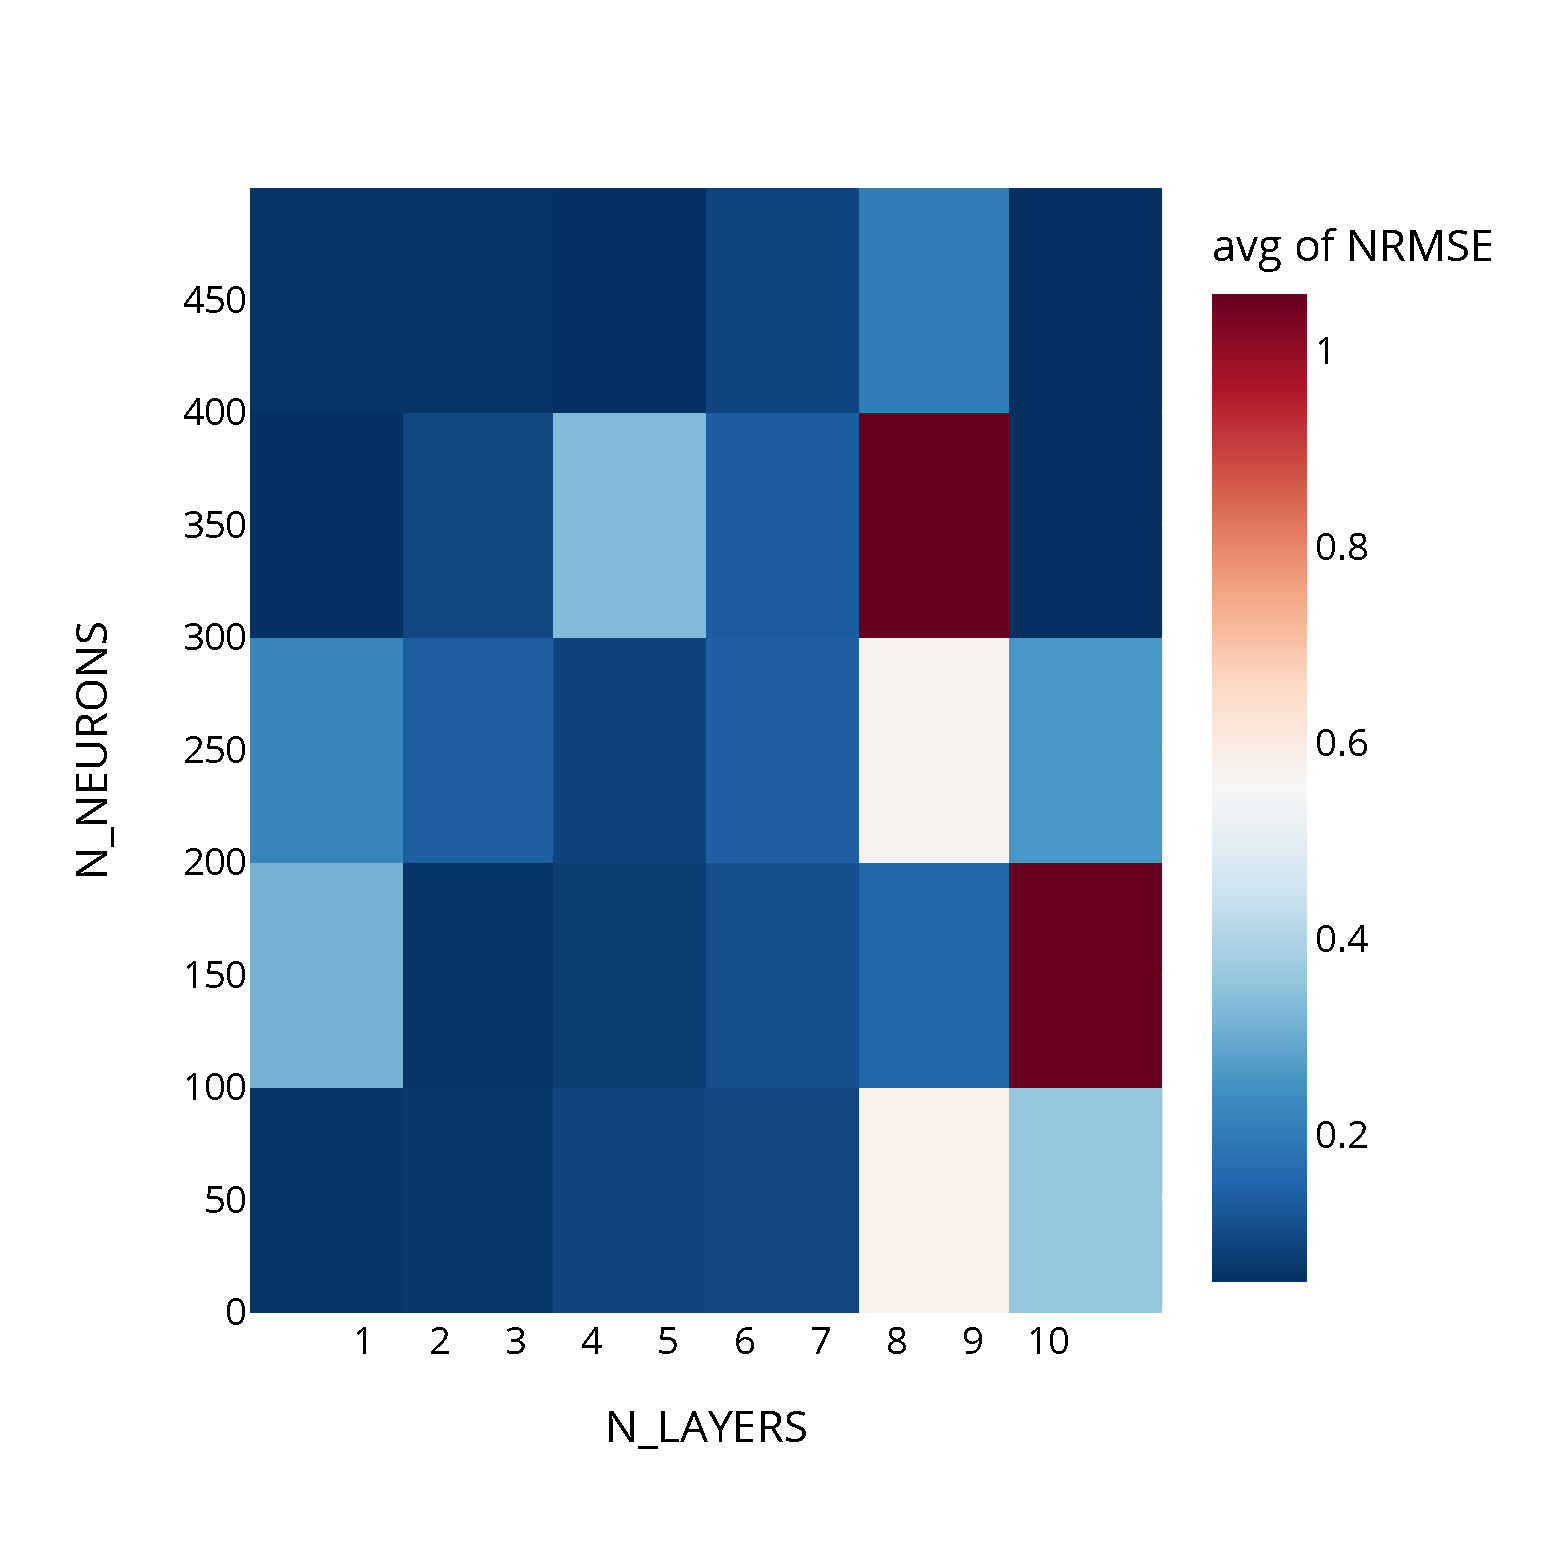
\includegraphics[width=\linewidth]{Figuras/hpo/hpo_plots_#1_#2/neurons_layers_heat_map_NRMSE.pdf}  
        \caption{NRMSE.}
        \label{fig:hpo_map_NRMSE_all_all}
    \end{subfigure}
    \begin{subfigure}{0.3\textwidth}
        \centering
        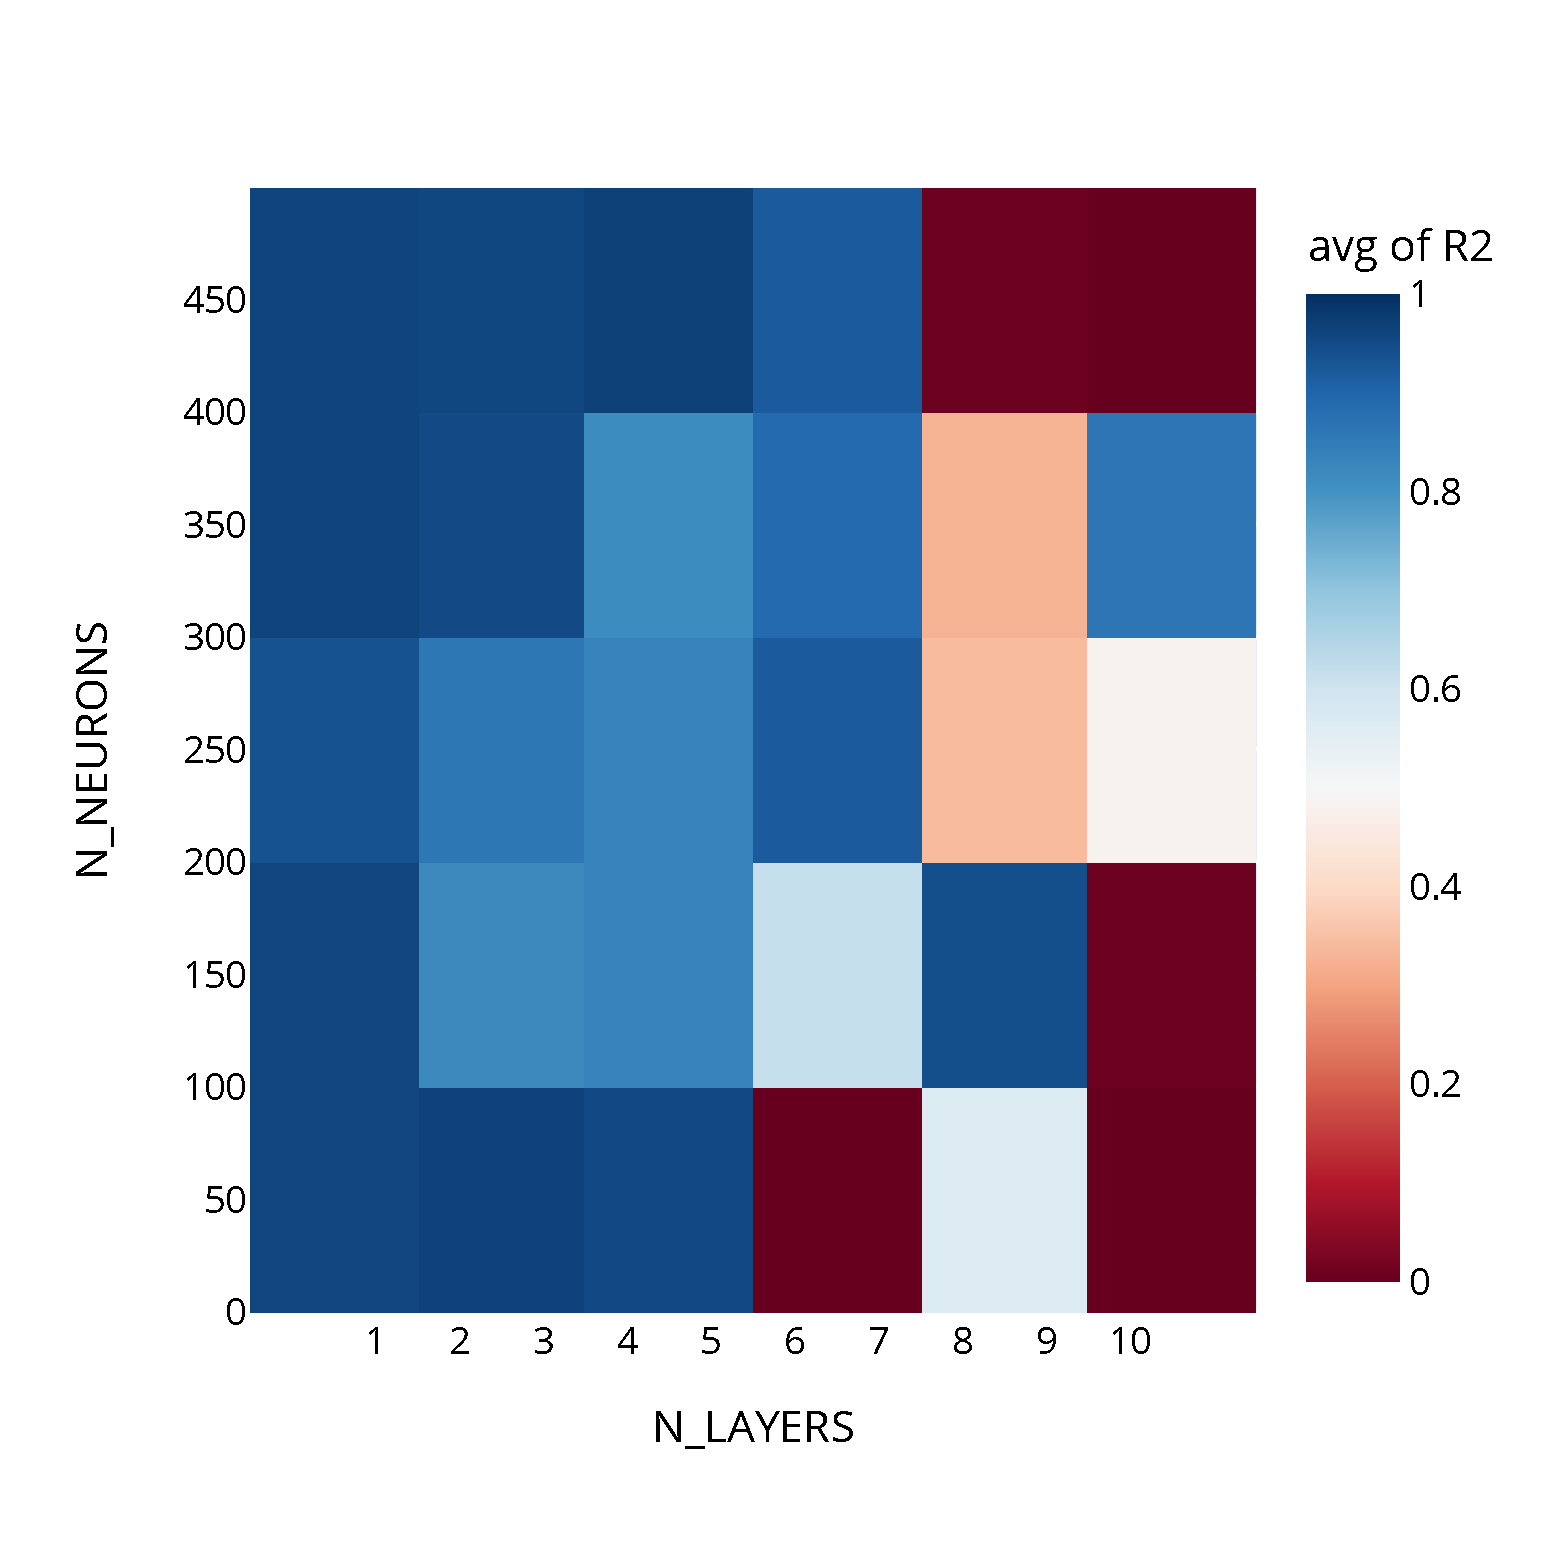
\includegraphics[width=\linewidth]{Figuras/hpo/hpo_plots_#1_#2/neurons_layers_heat_map_R2.pdf}  
        \caption{R2}
        \label{fig:hpo_map_R2_all_all}
    \end{subfigure}
    \caption{#3}
    \label{fig:hpo_map_all_all}
\end{figure}
}

\newcommand{\plothpohistogram}[3]{
\begin{figure}[t]
    \centering
    \begin{subfigure}{0.3\textwidth}
        \centering
        % include second image
        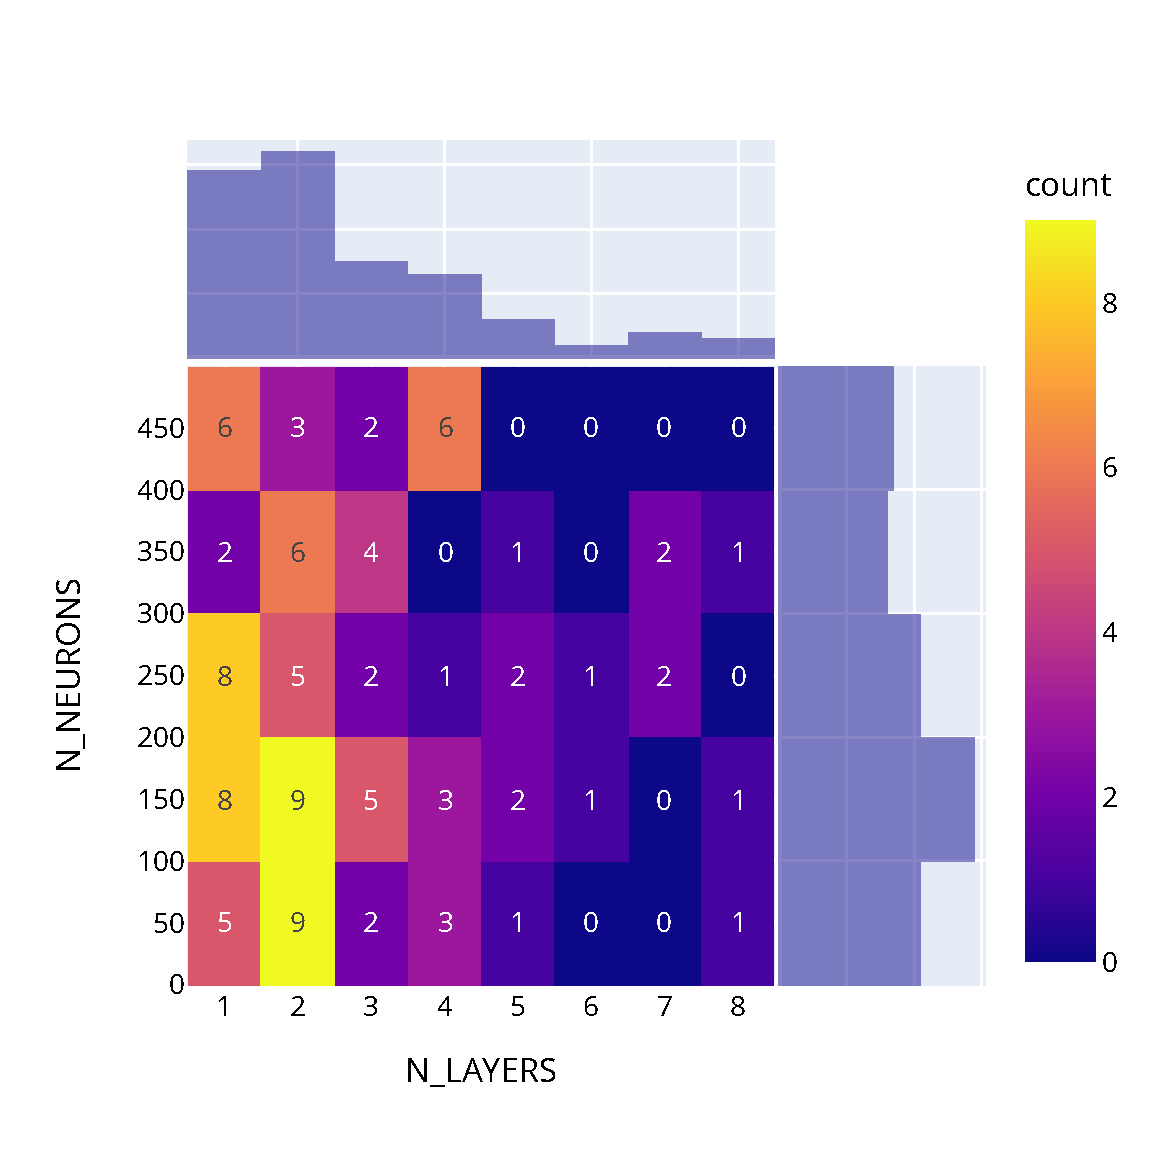
\includegraphics[width=\linewidth]{Figuras/hpo/hpo_plots_#1_#2/hpo_nn_hist_neurons_layers.pdf}  
        \caption{Histogram neurons layers.}
        \label{fig:hpo_hist_neurons_#1_#2}
    \end{subfigure}
    \begin{subfigure}{0.3\textwidth}
        \centering
        % include second image
        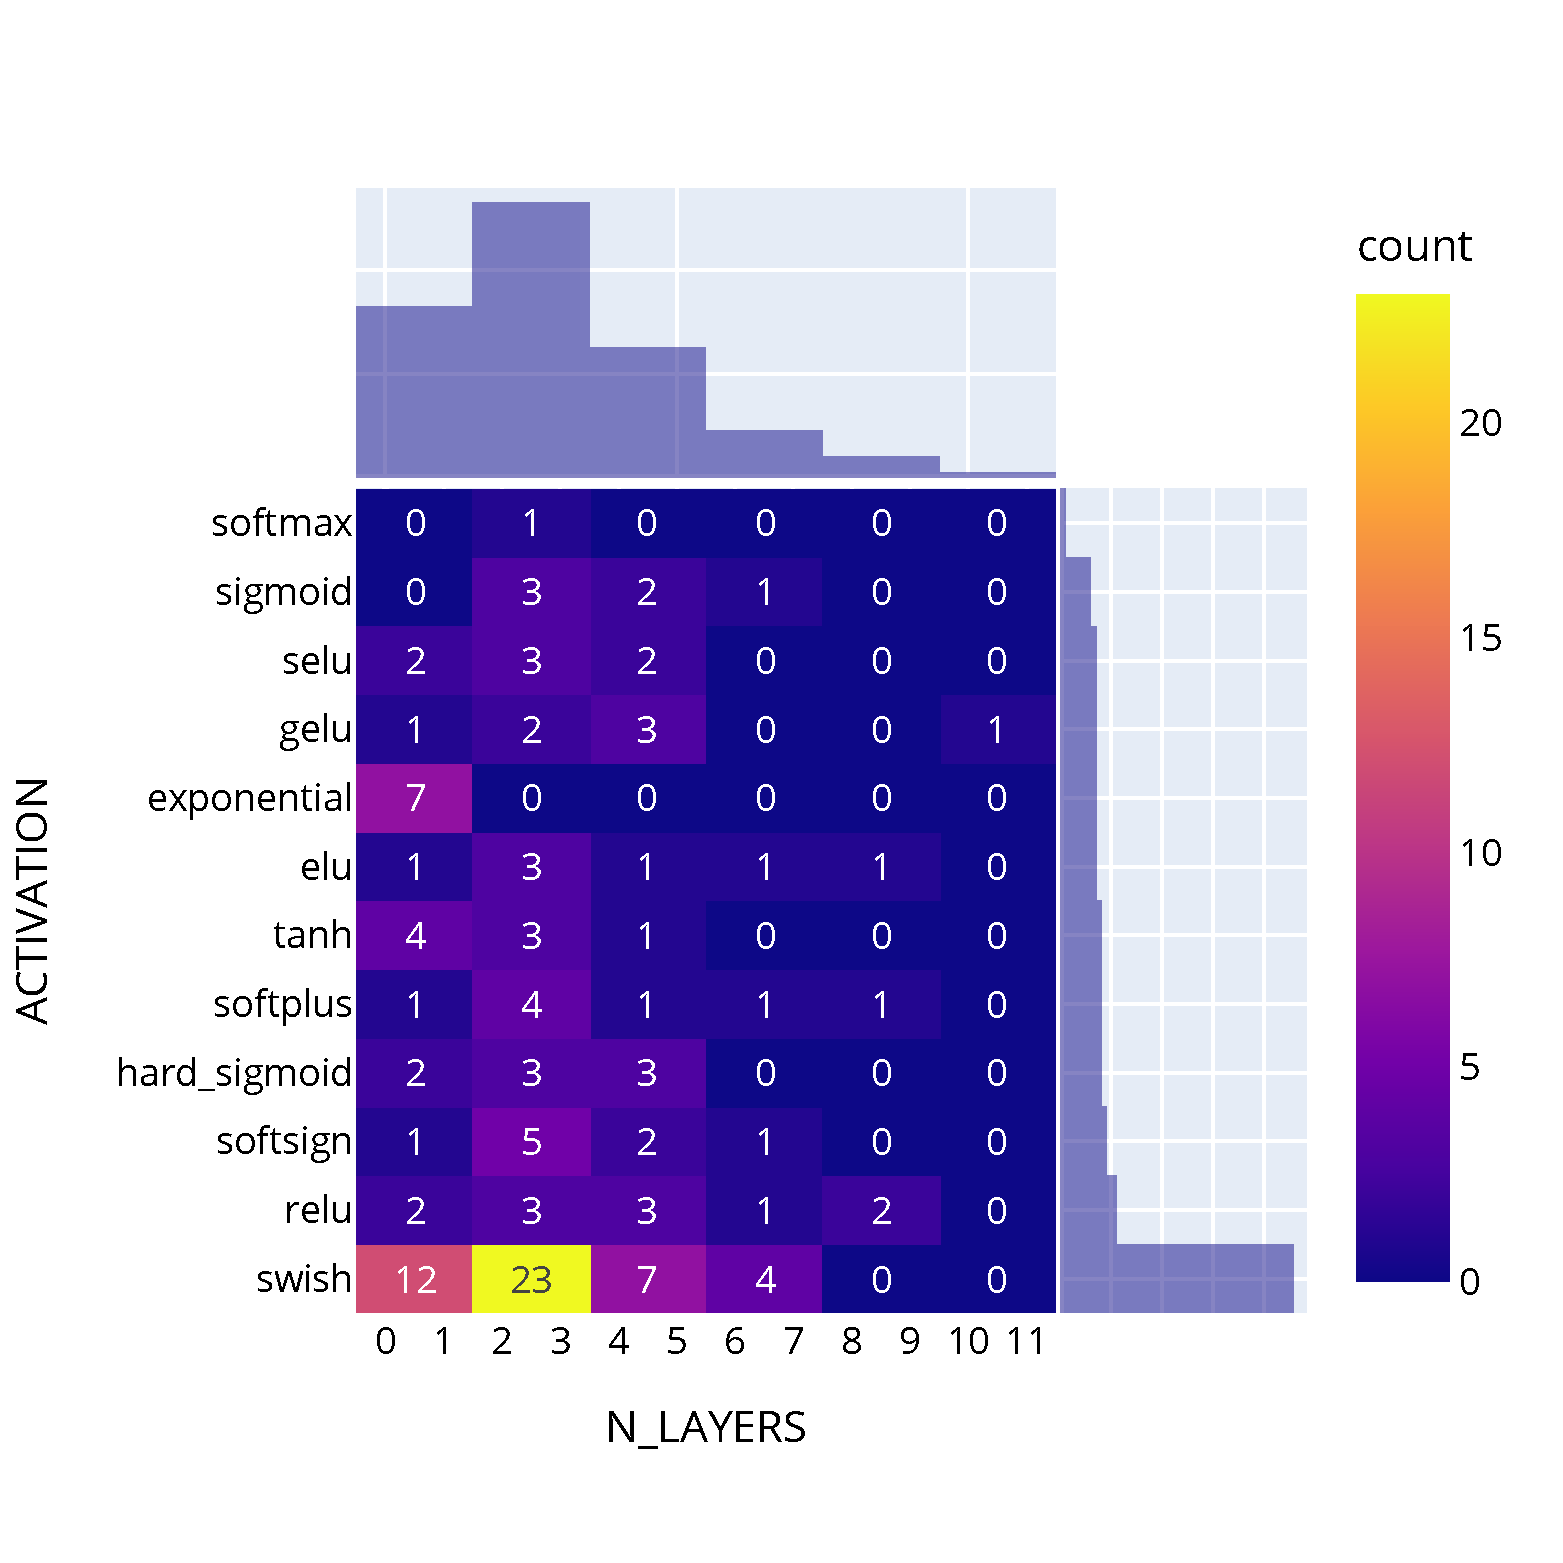
\includegraphics[width=\linewidth]{Figuras/hpo/hpo_plots_#1_#2/hpo_nn_activation_layers_count.pdf}  
        \caption{Histogram activation layers.}
        \label{fig:hpo_hist_activation_#1_#2}
    \end{subfigure}
    \begin{subfigure}{0.3\textwidth}
        \centering
        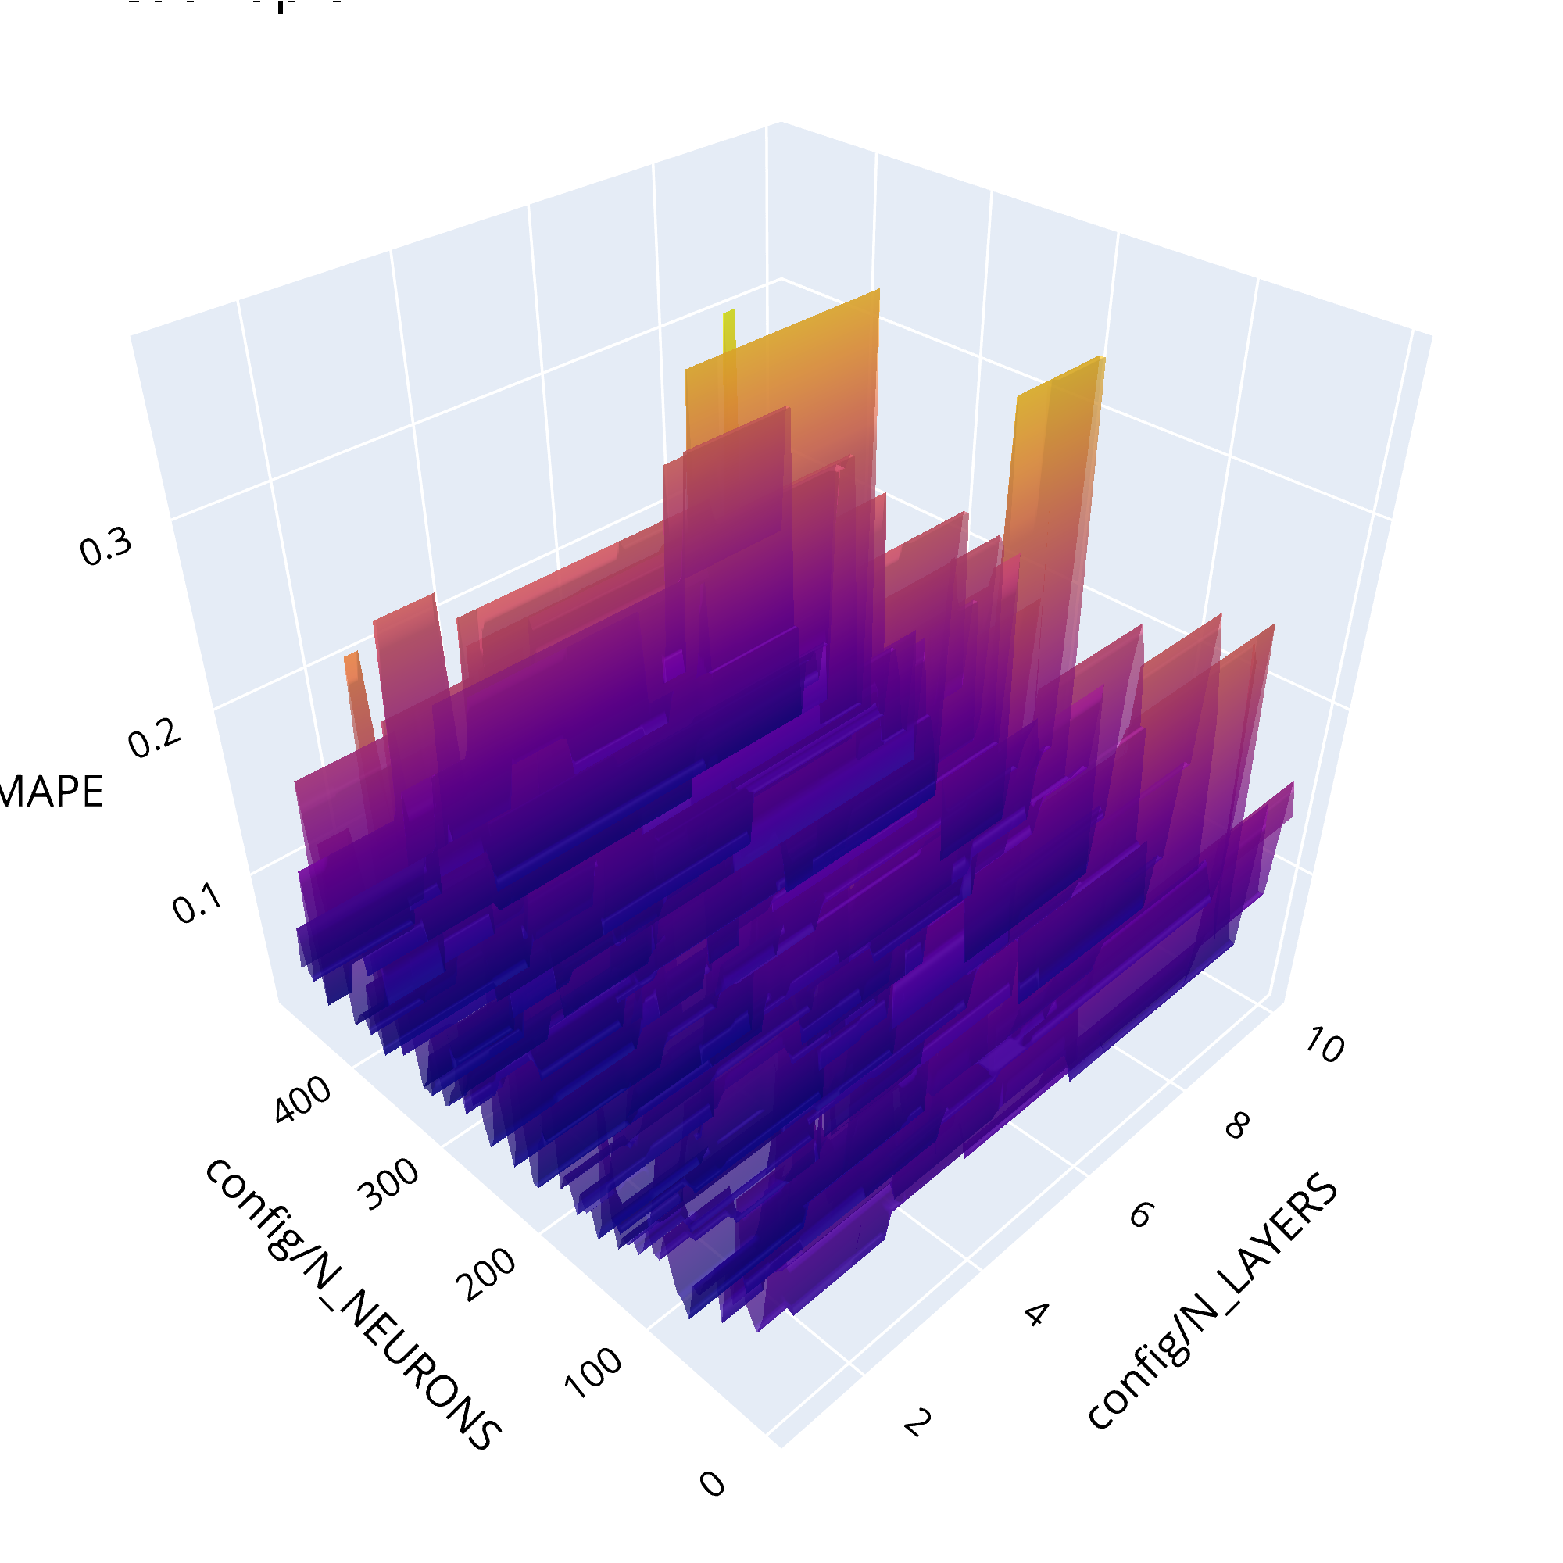
\includegraphics[width=\linewidth]{Figuras/hpo/hpo_plots_#1_#2/hpo_nn_activation_layers_surface.pdf}  
        \caption{Surface MAPE}
        \label{fig:hpo_surface_MAPE_#1_#2}
    \end{subfigure}
    \caption{#3}
    \label{fig:hpo_hist_#1_#2}
\end{figure}
}
%% =============================
%%      IMPORTANTE
%% ESTE ARQUIVO DEVE ESTAR SALVO COMO
%%      UTF - 8
%% =============================

% ----------------------------------------------------------
% Este capítulo é parte integrante do arquivo mestre
% Relatorio_TCC_Mestrado_Base_VERSÃO_SUBVERSÃO
% Formatos com \caption acima do \includegraphics conforme ABNT
% ----------------------------------------------------------

% -----------------------------------------
% Metodologia
%
% A ideia é utilizar a mesma sequência de entrada ter a opção de trocar a posição conforme a necessidade
% 
% O comando deve ser usado dentro do ambiente {figure} de forma que o comando \label{key} esteja dentro do ambiente e permita a melhor localização pelo editor LaTeX
%
% Forma de uso
%
% --------------------- Figuras Simples
%	\begin{figure}[H]
%		\figNameCommand{options includegraphics}{filename with path}{caption}
%		\label{label_figure_1}
%	\end{figure}
%
% --------------------- Figuras Compostas
%	\begin{figure}[H]
%		\figCapTwoSubfigInc{caption geral}
%		{subcaption (a) }
%		{width = 7cm, height = 6cm, trim = 0cm 0cm 0cm 0cm, clip = true}
%		{figure with path}
%		{subcaption (b) }
%		{width = 7cm, height = 6cm, trim = 0cm 0cm 0cm 0cm, clip = true}
%		{figure with path}
%		\label{fig_label}
%	\end{figure}
%
% --------------------- Comando Trim
% trim = left bottom right top
% -----------------------------------------

% -----------------------------------------
% Comandos para Figuras Simples
% -----------------------------------------
\newcommand{\figIncLongCap}[3]
{ 	
	\centering
	\caption{#3}
	\includegraphics[#1]{#2}
}

\newcommand{\figIncShortCap}[4]
{ 	
	\centering
	\caption[#4]{#3}
	\includegraphics[#1]{#2}
}

% -----------------------------------------
% Comandos para Figuras Duplas Com Subfigures
% -----------------------------------------
\newcommand{\figTwoSubfigIncLongCap}[7]
{ 	
	\centering
	\caption{#7}
	\subfigure[#1]
	{\includegraphics[#2]{#3}}
	\quad
	\subfigure[#4]
	{\includegraphics[#5]{#6}}
}

\newcommand{\figTwoSubfigIncShortCap}[8]
{ 	
	\centering
	\caption[#8]{#7}
	\subfigure[#1]
	{\includegraphics[#2]{#3}}
	\quad
	\subfigure[#4]
	{\includegraphics[#5]{#6}}
}

% -----------------------------------------
% Comandos para Figuras Triplas em Cascata Com Subfigures
% -----------------------------------------
\newcommand{\figThreeSubfigIncCap}[4]
{ 	
	\centering
	\SubfigSubcapSubfigInc{#1}
	\quad
	\SubfigSubcapSubfigInc{#2}
	\quad
	\SubfigSubcapSubfigInc{#3}
	\quad
	\caption{#4}
}

% -----------------------------------------
% Comandos Base para Figuras Múltiplas em Cascata Com Subfigures
% -----------------------------------------
\newcommand{\SubfigcapSubfigInc}[3]
{ 	
	\subfigure[#1]
	{\includegraphics[#2]{#3}} 
}

%%%%%%%%%%%%%%%%%%%%%%%%%%%%%%%%%%
% ===== Magno old versions ===== %
%%%%%%%%%%%%%%%%%%%%%%%%%%%%%%%%%%

% -----------------------------------------
% Comandos para Figuras Duplas sem Subfigure
% -----------------------------------------
\newcommand{\figDob}[5]
{   
	\centering
	\caption{#5}
	\includegraphics[#1]{#2}
	\includegraphics[#3]{#4} \\
	\vspace*{0.2cm}
	(a) \hspace{6.5cm} (b)
}

% -----------------------------------------
% Comandos para Figuras Triplas sem Subfigure
% -----------------------------------------
\newcommand{\figTre}[7]
{   
	\centering
	\caption{#7}
	\includegraphics[#1]{#2}
	\includegraphics[#3]{#4} \\
	\vspace*{0.2cm}
	(a) \hspace{6.5cm} (b) \\
	\includegraphics[#5]{#6} \\
	\vspace*{0.2cm}
	(c)
}

\newcommand{\figTreV}[7]
{   
	\centering
	\caption{#7}
	\includegraphics[#1]{#2}
	\includegraphics[#3]{#4}
	\includegraphics[#5]{#6}   \\
	\vspace*{0.2cm}
	(a) \hspace{4.cm} (b) \hspace{4.cm} (c)
}
% ----------------------------------------------------------
% Fim Arquivo
% ==========

% ==========  Seleção de uso de links coloridos para visualização ou sem cor para impressão final
\togglefalse{LinksComCores} 		% Opção links SEM CORES => Forma correta para imprimir a versão final a ser entregue
% ==========

% ========== Pacotes
%% =============================
%%      IMPORTANTE
%% ESTE ARQUIVO DEVE ESTAR SALVO COMO
%%      UTF - 8
%% =============================

% ----------------------------------------------------------
% Este capítulo é parte integrante do arquivo mestre
% Relatorio_TCC_Mestrado_Base_VERSÃO_SUBVERSÃO
% ----------------------------------------------------------
\usepackage{natbib}
\usepackage[T1]{fontenc}
%\usepackage[latin1]{inputenc}
\usepackage[utf8]{inputenc}
% =========
\usepackage{pgfplots}
\usepackage{tabularx}
% -----------------------------------------
% Pacotes básicos 
% -----------------------------------------
\usepackage[section]{placeins}
\usepackage{lastpage}		% Usado pela Ficha catalográfica
\usepackage{indentfirst}	% Indenta o primeiro parágrafo de cada seção.
\usepackage{color}			% Controle das cores
\usepackage{microtype} 		% Melhorias de justificação \usepackage[section]{placeins}
% \usepackage{amsmath} 		% Referências de equações com parênteses automático usar \eqref
\usepackage{physics,amsmath}

\usepackage{amssymb} 		% Símbolos matemáticos, incluindo os principais conjuntos numéricos
\usepackage{cancel}
% -----------------------------------------

% -----------------------------------------
% Pacotes gráficos
% -----------------------------------------
\usepackage{ae}
\usepackage{aecompl}
\usepackage{graphicx, import}	% Inclusão de gráficos
\usepackage{float} 		% Permite que eu use "H" para a figura ficar entre os parágrafos que eu quero
%\usepackage{subfigure} % make it possible to include more than one captioned figure/table in a single float
%\usepackage[font=small,labelfont=bf]{caption}
\usepackage[font=footnotesize]{caption} % Reduz o tamanho de todos os ``captions''
%\usepackage{subcaption}
%\usepackage{subfloat} % make it possible to include more than one captioned 
\usepackage{epstopdf}
\usepackage{ulem}
\usepackage{nomencl}
\makenomenclature
% \usepackage{framed}
\usepackage{lipsum} % geração de texto inútil - dummy
\usepackage{morefloats}

% -----------------------------------------
% Pacotes gráficos - Formatação do título
% -----------------------------------------
% Se fncychap for adicionado como RequirePackage dentro de ufabcFHZ#.cls não gera o mesmo efeito.
\usepackage[Bjornstrup]{fncychap} % Formas elegantes de cabeçalho
%% ------------------------------------
% Referência: http://tex.stackexchange.com/questions/13357/fncychap-package-reduce-vertical-gap-space-between-header-and-chapter-heading
%% ------------------------------------
%% A única alteração feita é em ``\vspace'', por padrão será usado ``-1cm'', fica bom, maximiza o espaço  - Não é necessário editar esse trecho.
%% ------------------------------------
\makeatletter
\renewcommand*{\@makechapterhead}[1]{%
	%\vspace*{-5\p@}%
	\vspace*{-1cm}% Recuo vertical para maximizar aproveitamento da página
	{\parindent \z@ \raggedright \normalfont
		\ifnum \c@secnumdepth >\m@ne
		\if@mainmatter%%%%% Fix for frontmatter, mainmatter, and backmatter 040920
		\DOCH
		\fi
		\fi
		\interlinepenalty\@M
		\if@mainmatter%%%%% Fix for frontmatter, mainmatter, and backmatter 060424
		\DOTI{#1}%
		\else%
		\DOTIS{#1}%
		\fi
	}
}
% For the case \chapter*:
\renewcommand*{\@makeschapterhead}[1]{%
	\vspace*{-1cm}% Recuo vertical para maximizar aproveitamento da página
	{\parindent \z@ \raggedright
		\normalfont
		\interlinepenalty\@M
		\DOTIS{#1}
		\vskip 40\p@
	}
}
\makeatother
%% ------------------------------------

% -----------------------------------------
% Pacotes Ambiente de comentário
% -----------------------------------------
\usepackage{comment}

% ----------------------------------------- 
% Tabelas
% ----------------------------------------- 
\usepackage{booktabs} % for much better looking tables
\usepackage{multirow} % Permite uma célula de várias linhas
% ----------------------------------------- 

% ----------------------------------------- 
% Enumerate com letras pré-fixas
% ----------------------------------------- 
\usepackage{paralist} 		% very flexible & customisable lists (eg. enumerate/itemize, etc.)
\usepackage{enumitem}

% ----------------------------------------- 
% Equações
% ----------------------------------------- 
\usepackage{breqn} 		 % Garante quebra automático com \begin{dmath}, mesmo contador de \begin{equation}
\usepackage{array} 		 % for better arrays (eg matrices) in maths
\usepackage{subeqnarray} % Permite o use de subnumeração numa equação 1.a 1.b 1.c etc
\usepackage{cancel} 	 % Permite o corte numa simplificação de expressão:
% \cancel{expression}
% \cancelto{value}{expression}

% ----------------------------------------- 
% Links Coloridos - Com seleção de uso de cores pelo usuário no arquivo base usando \toogletrue ou \togglefalse
% ----------------------------------------- 
\usepackage[colorlinks=true,
linkcolor 		= red,
anchorcolor 	= black,
citecolor 		= green,
filecolor 		= cyan,
	% ==== Selecionando opção de links coloridos - Em parceria com comando "\newtoggle{LinksComCores}"
	\iftoggle{LinksComCores}{%
		%hidelinks
	}{%
		hidelinks
	}
	% ==== 
]{hyperref} %Pacote para hyperlinks
%hidelinks %opção para os links não serem coloridos, útil para a versão final do trabalho, também posso usar %linkcolor=black


% ----------------------------------------- 
% Links Coloridos - Com seleção de uso de cores (des)comentando "hidelinks"
%% - Este código está dentro da classe ufabcFHZ#.cls
%% - 	Ele é mantido aqui para conferência
% ----------------------------------------- 
%\usepackage[colorlinks=true,
%linkcolor 		= red,
%anchorcolor 	= black,
%citecolor 		= green,
%filecolor 		= cyan,
%hidelinks
%]{hyperref} %Pacote para hyperlinks
%%hidelinks %opção para os links não serem coloridos, útil para a versão final do trabalho, também posso usar %linkcolor=black

% ----------------------------------------- 
% Inserção de código do Matlab
% ----------------------------------------- 
\usepackage[numbered]{mcode} 		% configure listings for Matlab

%==== Pacote para url nas referências da ABNT
%\usepackage[num,abnt-url-package=url]{abntcite}
%====

% for subfigures
\usepackage{caption}
\usepackage{subcaption}
\usepackage{capt-of}

% to draw circuits
\usepackage{circuitikz}
\usepackage{tikz}

\usepackage{makecell}
% ----------------------------------------------------------
% Fim Arquivo

\usetikzlibrary{shapes.geometric,arrows.meta}
\usetikzlibrary{positioning}
\usetikzlibrary{calc}
\usetikzlibrary{backgrounds}
\usetikzlibrary{fit}

\tikzstyle{diam} = [diamond, aspect=2, draw, fill=red!40, text width=6em,text centered ]
\tikzstyle{block} = [rectangle, draw, fill=blue!20, text width=3cm,text centered, rounded corners, minimum height=2em ]
\tikzstyle{trap} = [trapezium, trapezium left angle=70, trapezium right angle=110, minimum height=2em, text centered, draw=red, fill=green!30]
\tikzstyle{rect} = [rectangle, minimum width=3cm, minimum height=1cm, text centered, draw=red, fill=orange!30]
\tikzstyle{line} = [draw, -latex]


% for pseudo codes
\usepackage{algorithm}
\usepackage[noend]{algpseudocode}

\makeatletter
\newcommand*{\algrule}[1][\algorithmicindent]{%
  \makebox[#1][l]{%
    \hspace*{.2em}% <------------- This is where the rule starts from
    \vrule height .75\baselineskip depth .25\baselineskip
  }
}
\newcount\ALG@printindent@tempcnta
\def\ALG@printindent{%
    \ifnum \theALG@nested>0% is there anything to print
    \ifx\ALG@text\ALG@x@notext% is this an end group without any text?
    % do nothing
    \else
    \unskip
    % draw a rule for each indent level
    \ALG@printindent@tempcnta=1
    \loop
    \algrule[\csname ALG@ind@\the\ALG@printindent@tempcnta\endcsname]%
    \advance \ALG@printindent@tempcnta 1
    \ifnum \ALG@printindent@tempcnta<\numexpr\theALG@nested+1\relax
    \repeat
    \fi
    \fi
}
% the following line injects our new indent handling code in place of the default spacing
\patchcmd{\ALG@doentity}{\noindent\hskip\ALG@tlm}{\ALG@printindent}{}{\errmessage{failed to patch}}
\patchcmd{\ALG@doentity}{\item[]\nointerlineskip}{}{}{} % no spurious vertical space
% end vertical rule patch for algorithmicx
\makeatother

% mathcal lowerletters
%\usepackage{dutchcal}

%% =============================
%%      IMPORTANTE
%% ESTE ARQUIVO DEVE ESTAR SALVO COMO
%%      UTF - 8
%% =============================

% ----------------------------------------------------------
% Este capítulo é parte integrante do arquivo mestre
% Relatorio_TCC_Mestrado_Base_VERSÃO_SUBVERSÃO
% ----------------------------------------------------------


%================ Pacotes para inserir código
% ----------------------------------------- 
% Inserção de código do Matlab
% ----------------------------------------- 
\usepackage[numbered]{mcode} 		% configure listings for Matlab

% Deve estar na mesma pasta que o arquivo Base do relatório
%%%% *** Bloco adicionado em mcode.sty - FHZ
% % general definitions
% \lstset{%
% extendedchars = true,
% inputencoding = latin1, % funciona com latin1
%%%% ***

% ----------------------------------------- 
% en­ables the user to type­set pro­grams (pro­gram­ming code) 
% ----------------------------------------- 
\usepackage{listings}

%%%%% ++++++ Referências e explicações:
%http://tex.stackexchange.com/questions/68356/how-to-create-conditionals-in-a-document-class-for-latex
%http://tex.stackexchange.com/questions/30512/how-to-insert-code-with-accents-with-listings
%http://tex.stackexchange.com/questions/24528/having-problems-with-listings-and-utf-8-can-it-be-fixed
%http://tex.stackexchange.com/questions/30512/how-to-insert-code-with-accents-with-listings
%http://tex.searchalleasy.com/q/30512
%http://stackoverflow.com/questions/1116266/listings-in-latex-with-utf-8-or-at-least-german-umlauts
%http://www.mathworks.com/matlabcentral/fileexchange/8015-m-code-latex-package
%%%%% ++++++ 

% ----------------------------------------- 
% --- Comando para definir estilo da \lstinputlisting
% ----------------------------------------- 
\lstset{basicstyle=\footnotesize}

% ----------------------------------------- 
% --- Comando para garantir acentuação correta para \lstinputlisting[language = C].
% ----------------------------------------- 
\lstset{literate = %
	{Ö}{{\"O}}1
	{Ä}{{\"A}}1
	{Ü}{{\"U}}1
	{ß}{{\s{s}}}1
	{ü}{{\"u}}1
	{ä}{{\"a}}1
	{ö}{{\"o}}1
	{~}{{\textasciitilde}}1
	{ã}{{\~a}}1
	{á}{{\'a}}1
	{à}{{\`a}}1
	{â}{{\^a}}1
	{é}{{\'e}}1
	{ê}{{\^e}}1
	{í}{{\'\i}}1
	{õ}{{\~o}}1
	{ó}{{\'o}}1
	{ô}{{\^o}}1
	{ú}{{\'u}}1
	{ç}{{\c c}}1
	{Ã}{{\~A}}1
	{Á}{{\'A}}1
	{À}{{\`A}}1
	{Â}{{\^A}}1
	{É}{{\'E}}1
	{Ê}{{\^E}}1
	{Í}{{\'{I}}}1
	{Õ}{{\~O}}1
	{Ó}{{\'O}}1
	{Ô}{{\^O}}1
	{Ú}{{\'U}}1
	{Ç}{{\c {C}}}1
}
%================

% ----------------------------------------------------------
% Fim Arquivo
\usepackage{textcomp} % Fixes TS1 font shape for textbullet
% ========== 

% ========== Caminho das Figuras
\graphicspath{Figuras/}

% ------------------------------------------
% Cria Lista de Símbolos
% ------------------------------------------
\makelosymbols

% ------------------------------------------
% Cria Lista de Abreviações
% ------------------------------------------
\makeloabbreviations

% ------------------------------------------
% Início do documento
% ------------------------------------------
\begin{document}

% -----------------------------------------
% INFORMAÇÕES E DADOS - CAPA e FOLHA DE ROSTO
% -----------------------------------------
\title{Reduced Order Models for Parametric Domains: A Data-Driven Methodology for the Acceleration of Engineering Simulations}
\foreigntitle{Modelos de Ordem Reduzida para Domínios Paramétricos: Uma Metodologia Orientada por Dados para a Aceleração de Simulações em Engenharia}
\author{}{Allan Moreira de Carvalho}

% ------- Orientador e (se houver) Coorientador
\advisor{Prof. Dr.}{Daniel}{Jonas Dezan}{}
\advisor{Prof. Dr.}{Wallace}{Gusmão Ferreira}{}
\advisor{Prof. Dr.}{Alberto}{Costa Nogueira Junior}{}

% ------- Banca
\examiner{Prof. Dr.}{Marcia Maria Penteado Marchesini}{External Examiner}
\examiner{Prof. Dr.}{Wilson Carlos da Silva Júnior}{External Examiner}
\examiner{Prof. Dr.}{Franciane Freitas Silveira}{Internal Substitute Examiner}
\examiner{Prof. Dr.}{Rômulo Gonçalves Lins}{Chair}
% ------- Coordenador do curso
\coordinator{Prof.}{Dr.}{NomeCoordenador}{}
% ------ Data de entrega
\date{10}{07}{2025} % dia - mês - ano
% ------ Limite de 5 palavras chaves para ficha catalográfica
\keyword{Reduced Order Model}
\keyword{Machine Learning}
\keyword{Proper Orthogonal Decomposition (POD)}
\keyword{Parametric Modeling}
\keyword{Geometric Morphing}

% ------ Curso/Programa de pós-graduação
\department{EEN}

% ------------------------------------------
% Criar Capa
% ------------------------------------------
\maketitle

% -----------------------------
% ELEMENTOS PRÉ-TEXTUAIS
% -----------------------------
\frontmatter

% Dedicatória
\dedication{I dedicate it...}

% ------------------------------------------
% AGRADECIMENTOS - Input externo
% ------------------------------------------
\begin{agradecimentos}
	\vspace{5 mm}
    I thank to...
\end{agradecimentos}
% -----------------------------------------

% -----------------------------------------
% EPÍGRAFE - Input externo
% -----------------------------------------
\begin{epigrafe}
    \vspace*{\fill}
    \begin{flushright}
    \textit{``Learn from the mistakes of those who followed your advice'' \\ (Unknown author)}
    \end{flushright}
\end{epigrafe}

% --- resumo em inglês
\begin{foreignabstract}
This dissertation introduces a comprehensive and adaptable framework for the construction of data-driven, parametric reduced-order models (ROMs) to accelerate the analysis of complex physical systems. High-fidelity numerical simulations, while accurate, impose a prohibitive computational cost in multi-evaluation scenarios such as design optimization, uncertainty quantification, and real-time control. To overcome this bottleneck, this work develops a unified pipeline that combines techniques in data preprocessing, dimensionality reduction, and machine learning. The core methodology employs Proper Orthogonal Decomposition (POD) to extract dominant, energy-optimal spatial modes from high-dimensional simulation snapshot data, which are then mapped from the design parameters using regression models like Gaussian Process Regression (GPR) or Artificial Neural Networks (ANNs). A critical innovation, developed to address challenges with complex geometries, is a sophisticated technique for handling geometric variations, which ensures topological consistency across differing parametric domains.

The framework's efficacy was first established in a 2D context by conducting a comparative analysis of POD-GPR and POD-ANN models for the reconstruction of supersonic nozzle flows, which are characterized by strong shock-wave/boundary-layer interactions. This initial study introduced a novel hybrid loss function for ANN training and employed SHapley Additive exPlanations (SHAP) to enhance model interpretability. However, the subsequent challenge of applying the framework to a complex 3D case—the parametric reconstruction of pressure and temperature fields on the blade surfaces of the NASA Rotor 37—revealed a fundamental limitation: meshes of varying sizes and inconsistent topologies prevented the direct application of POD. This problem necessitated the development of the aforementioned geometric mesh morphing technique, which proved crucial for enabling the methodology's extension to variable 3D shapes.

Results from both studies demonstrate exceptional predictive accuracy, with coefficients of determination ($R^2$) consistently exceeding 0.95, and computational speed-ups of several orders of magnitude (50x to over 10,000x) compared to full-fidelity simulations. This work not only provides a robust and validated methodology for accelerating simulation-based design and analysis cycles but also offers practical guidelines on model selection and training, establishing a foundation for the next generation of intelligent simulation tools.
\end{foreignabstract}
\keywordeng{Reduced Order Model};
{Machine Learning};
{Proper Orthogonal Decomposition (POD)};
{Parametric Modeling};
{Geometric Morphing}

% --- resumo em português
\begin{abstract}
Esta dissertação introduz um framework abrangente e adaptável para a construção de modelos de ordem reduzida (ROMs) paramétricos e orientados por dados, visando acelerar a análise de sistemas físicos complexos. Simulações numéricas de alta fidelidade, embora precisas, impõem um custo computacional proibitivo em cenários de que necessitam de múltiplas avaliações, como otimização de forma, quantificação de incertezas e controle em tempo real. Para superar esse gargalo, este trabalho desenvolve um pipeline unificado que combina técnicas de pré-processamento de dados, redução de dimensionalidade e aprendizagem de máquina. A metodologia central emprega a Decomposição Ortogonal Própria (POD) para extrair modos espaciais dominantes, que são então mapeados a partir dos parâmetros de projeto usando modelos de regressão como a Regressão por Processo Gaussiano (GPR) ou Redes Neurais Artificiais (ANNs). Uma inovação crítica, desenvolvida para lidar com geometrias complexas, é uma técnica sofisticada para o tratamento de variações geométricas, que garante a consistência topológica entre diferentes domínios paramétricos.

A eficácia do framework foi primeiramente estabelecida em um contexto 2D, através de uma análise comparativa de modelos POD-GPR e POD-ANN para a reconstrução de escoamentos em bocais supersônicos. Este estudo inicial introduziu uma função de perda híbrida para o treinamento da ANN e empregou SHapley Additive exPlanations (SHAP) para aumentar a interpretabilidade do modelo. No entanto, o desafio subsequente de aplicar o framework a um caso 3D—a reconstrução paramétrica dos campos de pressão e temperatura nas pás do NASA Rotor 37—revelou uma limitação fundamental: malhas com tamanhos distintos e topologias inconsistentes impediram a aplicação direta do POD. Este problema tornou necessário o desenvolvimento da técnica de tratamento geométrico usando deformação de malha, que se mostrou crucial para permitir a extensão da metodologia a formas 3D variáveis.

Os resultados de ambos os estudos demonstram excepcional precisão preditiva, com coeficientes de determinação ($R^2$) consistentemente acima de 0.95, e uma aceleração computacional de várias ordens de magnitude (de 50x a mais de 10.000x) em comparação com as simulações de alta fidelidade. Este trabalho não apenas fornece uma metodologia robusta e validada para acelerar os ciclos de projeto e análise baseados em simulação, mas também oferece diretrizes práticas quanto a seleção e o treinamento de modelos, estabelecendo a base para a próxima geração de ferramentas de simulação inteligentes.
\end{abstract}
\palavrachave{Modelo de Ordem Reduzida};
{Aprendizado de Máquina};
{Decomposição Ortogonal Própria (POD)};
{Modelagem Paramétrica};
{Mapeamento de Malha}

% -----------------------------------------
% Inserir Lista de Figuras
% -----------------------------------------
\listoffigures

% -----------------------------------------
% Inserir lista de Tabelas
% -----------------------------------------
\listoftables

% -----------------------------------------
% Inserir lista de símbolos e abreviações
% -----------------------------------------
\printloabbreviations
\printlosymbols

% -----------------------------------------
% Inserir Sumário
% -----------------------------------------
\makeatletter \let\ps@plain\ps@empty \makeatother
\tableofcontents
% -----------------------------------------

\setcounter{pagenumber_frontmatter}{\number\value{page}}

% -----------------------------
% ELEMENTOS TEXTUAIS
% -----------------------------
\mainmatter

\iftoggle{toggleVersaoFinal}
{\setcounter{page}{\number\value{pagenumber_frontmatter} + 2}}
{\setcounter{page}{\number\value{pagenumber_frontmatter} + 1}}

% -----------------------------------------
% CAPÍTULOS
% -----------------------------------------

\chapter{Introduction}

\section{The Multi-Query Bottleneck in Computational Fluid Dynamics}

In the modern era of aerospace and turbomachinery engineering, Computational Fluid Dynamics (CFD) has become an indispensable tool for analysis and design \citep{Spalart2016}. High-fidelity numerical models, such as those based on the Reynolds-Averaged Navier-Stokes (RANS) equations, Large Eddy Simulation (LES), or even Direct Numerical Simulation (DNS), offer remarkable precision in predicting the behavior of fluid flows \citep{Pereira2021}. This capability allows engineers to investigate complex physical phenomena, from the turbulent wake behind an aircraft to the intricate shock structures within a supersonic engine, with a level of detail that is often hard to achieve through physical experimentation alone \citep{Schiestel2022}.

However, the high fidelity of these simulations comes at a price: computational expense. Solving the governing equations of fluid motion across complex geometries discretized into millions or even billions of grid cells requires immense computational resources and can take hours, days, or even weeks on high-performance computing (HPC) clusters \citep{slotnick2014cfd}. While the cost of a single simulation may be justifiable for final design verification, it becomes prohibitive in the context of the modern engineering design cycle. The core challenge is not merely that a single CFD simulation is slow, but that contemporary design and analysis workflows are inherently "multi-evaluation"-or "multi-query"-in nature \citep{Bekemeyer2025}.

Tasks such as design space exploration, aerodynamic shape optimization, uncertainty quantification (UQ), and sensitivity analysis require the evaluation of hundreds, if not thousands, of design variations \citep{Yondo2018}. For example, a gradient-based optimization algorithm may need to iteratively adjust dozens of geometric parameters to maximize lift or minimize drag, with each iteration demanding a new CFD simulation \citep{Kenway2016}. Similarly, a robust UQ analysis might involve propagating uncertainties from manufacturing tolerances or operational conditions through the model, a task that often relies on Monte Carlo methods requiring a vast number of simulations to achieve statistical convergence \citep{Smith2014}. When each model evaluation involves a computationally expensive CFD run, these essential engineering tasks become computationally intractable \citep{slotnick2014cfd}. This "multi-evaluation bottleneck" represents a fundamental barrier to innovation, slowing down the design cycle and limiting the ability of engineers to explore novel concepts or quantify risks effectively.

This research is directly motivated by these challenges, framed within the context of Project 77 - Design Optimization and Experimental Evaluation of Centrifugal Compressors for CO2 and CO2-CH4 Mixtures under Supercritical Conditions of the Research Centre for Greenhouse Gas Innovation (RCGI), a critical technologies for carbon capture, utilization, and storage (CCS) \citep{RCGI_Project77}. The path to simulating these complex machines requires a new methodology capable of handling representative physical phenomena—such as compressibility, high Reynolds numbers, turbulence, and complex geometric variations—in a computationally efficient manner.

\section{Reduced-Order Models (ROMs)}

To overcome the multi-evaluation bottleneck, a new paradigm is required, moving away from the direct, repeated use of high-fidelity models. The strategic solution lies in the development of surrogate models, also known as metamodels or response surfaces \citep{Hu2020}. A surrogate model is a computationally inexpensive, approximation of the complex, high-fidelity model. Data-driven surrogates learn the input-output relationship from a limited set of pre-computed high-fidelity simulations, providing near-instantaneous predictions for new design points, effectively replacing the expensive CFD solver within the multi-evaluation loop \citep{Yondo2018, EspinosaBarcenas2023}. This approach transforms an intractable problem into a feasible one, enabling fast design exploration and robust analysis without sacrificing the essential physical insights provided by the original high-fidelity data \citep{Hu2020}.

Among the various classes of surrogate models, data-driven Reduced-Order Models (ROMs) have emerged as a particularly powerful paradigm for high-dimensional physical systems like fluid flows. The central philosophy of ROMs is an "offline-online" computational strategy. In the offline, or "training," stage, a set of computationally expensive, high-fidelity simulations is performed to generate a database of "snapshots" of the system's behavior across a range of parameters. A fracation of this database is then used to train the ROM. Once trained, the ROM can be deployed in the online, or "prediction," stage, where it provides extremely fast approximations for new, unseen parameter inputs. This decouples the high computational cost of data generation from the rapid-query demands of the application.

The construction of a machine learning-based ROM (ML-ROM) for a parametric system typically follows a structured pipeline, which forms the backbone of this dissertation. This pipeline can be conceptualized in four primary stages:

\begin{itemize}
    \item Data Generation: A Design of Experiments (DoE) is created to strategically sample the parametric design space. A high-fidelity CFD solver is then run for each sample point to generate a database of high-dimensional solution snapshots.
    \item Dimensionality Reduction: The immense dimensionality of the snapshot data (often millions of degrees of freedom per snapshot) is reduced to a very low-dimensional latent space. This is typically achieved using techniques like Proper Orthogonal Decomposition (POD), which extracts a small set of dominant, energy-optimal basis functions, or "modes", that capture the essential dynamics or parametric sensitivity of the flow.
    \item Latent-Space Regression: A machine learning model (the surrogate regressor) is trained to learn the mapping between the low-dimensional input design parameters (e.g., blade angle, Mach number) and the low-dimensional latent-space representation (e.g., the POD mode coefficients) of the flow field.
    \item Field Reconstruction: During the online phase, the trained regressor predicts the latent-space coefficients for a new set of design parameters. These coefficients are then used to reconstruct the full, high-dimensional flow field through a linear combination of the pre-computed basis functions.
\end{itemize}

This structured approach allows for the systematic deconstruction of a complex modeling problem into a series of more manageable tasks, each addressable with specialized mathematical and computational tools.

% Adicionar Figura mostrando o pipeline de construcao do ML-ROM
\section{Thesis Objectives and Contributions}

The primary objective of this dissertation is to develop, validate, and analyze a unified, flexible, and robust framework for creating parametric reduced-order models for complex fluid dynamics problems. This work aims to move beyond ad-hoc solutions for specific problems and establish a comprehensive methodology that can be adapted to a wide range of challenges in computational aerodynamics, from internal supersonic flows to transonic turbomachinery. And also to addresses critical gaps in the existing literature. 

The research is structured as a progression of case studies with increasing complexity, chosen to be computationally tractable while serving as fundamental steps toward the final objective. The key contributions of this dissertation, which collectively advance the state-of-the-art in data-driven aerodynamic modeling, are as follows:

\begin{itemize}
    \item \textbf{A Unified and Validated Methodological Framework:} Developed a comprehensive, end-to-end computational pipeline for creating parametric ROMs. This reproducible framework integrates geometry parameterization, data generation, advanced mesh processing, POD, and machine learning regression (GPR and ANNs). Its versatility and robustness were rigorously validated across distinct and challenging flow regimes: a 2D supersonic nozzle with strong shock-wave interactions and a 3D transonic compressor blade.
    \item \textbf{Advanced Model Training and Physical Fidelity:} Introduced novel techniques to enhance the fidelity and trustworthiness of ANN-based ROMs:
        \begin{itemize}
            \item \textbf{A Differentiable, Physics-Informed Loss Function:} Developed a hybrid loss function that incorporates error from the reconstructed physical field directly into the training process. This acts as a physical regularizer, improving the capture of high-gradient features like shock waves without needing explicit PDE constraints.
            \item \textbf{Model Interpretability:} Employed SHapley Additive exPlanations (SHAP) to provide quantitative insight into the "black-box" models, linking their predictions to fundamental physical principles and building confidence in their results.
        \end{itemize}
    \item \textbf{Enabling Technology for Complex 3D Parametric ROMs:} Introduced and validated a mesh morphing technique based on harmonic mapping. This critical method resolves the fundamental challenge of topological inconsistency in parametric studies, enabling the direct application of POD to complex 3D geometries with varying shapes.
    \item \textbf{Integrated Geometry and Flow Field Prediction:} Developed a novel surrogate model that \textbf{simultaneously predicts both the high-dimensional aerodynamic fields and the underlying 3D physical geometry} from a single set of abstract design parameters. This addresses a major gap in the literature and is a significant step towards truly generative design.
    \item \textbf{Systematic Comparative Analysis for Model Selection:} Performed an in-depth, empirical comparison of GPR and ANN regressors. The analysis, supported by rigorous cross-validation and noise robustness studies, provides practical, evidence-based guidelines for selecting the appropriate surrogate model based on dataset size, data quality, and the complexity of the underlying physics.
\end{itemize}

\section{Dissertation Outline}

This dissertation is structured to guide the reader from foundational concepts to advanced applications and future possibilities.

\begin{itemize}
    \item \textbf{Chapter 2} provides a comprehensive review of the state-of-the-art, establishing the strategic context for this research by aligning it with the challenges of computational science and identifying specific gaps in the academic literature on reduced-order modeling.
    \item \textbf{Chapter 3} provides a comprehensive review of the theoretical foundations of reduced-order modeling and machine learning as applied to fluid dynamics, establishing the context and key concepts for the work.
    \item \textbf{Chapter 4} presents the first major case study, applying the framework to the parametric reconstruction of 2D supersonic nozzle flows, with a focus on the development of the hybrid loss function and a comparative analysis of surrogate regressors.
    \item \textbf{Chapter 5} presents the second case study, targeting the parametric reconstruction of 3D surface fields and geometry on the NASA Rotor 37, with a focus on the critical role of the mesh morphing technique.
    \item \textbf{Chapter 6} synthesizes the findings from both case studies, summarizes the key contributions of the dissertation, discusses its limitations, and proposes promising directions for future research.
\end{itemize}

\chapter{Literature Review of Reduced-Order Modeling and Machine Learning for Computational Fluid Dynamics}

\section{The Computational Bottleneck in High-Fidelity Turbomachinery Simulation}

The design and analysis of modern turbomachinery, from jet engines to power generation turbines, represent one of the most formidable challenges in computational engineering. The accurate prediction of aerodynamic and aero-thermal performance is paramount for achieving gains in efficiency, reliability, and safety, while reducing fuel consumption and environmental impact \citep{synthesized2024}. However, the physical environment within these machines is exceptionally complex, characterized by extreme conditions that push the boundaries of simulation capabilities.

\subsection{The Challenge of Simulating Complex Flow Physics}

Turbomachinery flows are inherently three-dimensional, unsteady, and turbulent, often operating in transonic or supersonic regimes \citep{synthesized2024}. These conditions give rise to a host of complex physical phenomena, including strong shock-wave/boundary-layer interactions, flow separation, secondary flows, and intense turbulence, all of which critically influence component performance and structural integrity \citep{synthesized2024, turbo_146_3_031009}. The accurate numerical simulation of such phenomena necessitates high-fidelity methods. Techniques like Large Eddy Simulation (LES) and Direct Numerical Simulation (DNS) offer detailed, time-resolved predictions of turbulent structures but come at a computational cost that is prohibitive for routine industrial design cycles, where hundreds or thousands of evaluations may be required \citep{synthesized2024, peherstorfer2018survey}. A single high-fidelity LES of a turbine vane, for example, can demand millions of CPU hours, rendering its use in many-query applications like design optimization infeasible \citep{peherstorfer2018survey}.

Consequently, the industry has historically relied on Reynolds-Averaged Navier-Stokes (RANS) simulations as the workhorse for aerodynamic design \citep{synthesized2024}. While computationally tractable, RANS methods introduce significant model-form uncertainty through the turbulence closure models they employ. These models often fail to accurately predict flows with significant separation, strong unsteadiness, or complex heat transfer, which are precisely the phenomena that limit turbomachinery performance \citep{synthesized2024, ijtpp-07-00016-v2}. This creates a persistent and challenging trade-off for engineers: the choice between computationally expensive simulations that are accurate but too slow for design exploration, and faster simulations that may lack the predictive fidelity required for high-stakes decisions \citep{synthesized2024}. This fidelity-cost dilemma forms the central motivation for the development of the advanced modeling techniques discussed in this review.

\subsection{The "CFD Vision 2030 Study" as a Community Roadmap}

The challenges facing the computational fluid dynamics (CFD) community were formally articulated in the landmark "CFD Vision 2030 Study," commissioned by NASA and authored by a multidisciplinary team led by Slotnick et al. \citep{slotnick2014cfd, park2016unstructured}. This report provided a knowledge-based forecast of future capability requirements and a strategic research roadmap to achieve a visionary CFD capability by the year 2030 \citep{slotnick2014cfd, turbo_146_3_031009}. The study identified several critical impediments that were preventing CFD from moving beyond a limited, albeit important, region of the design space to become a truly predictive tool across the full operational envelope \citep{park2016unstructured}.

A key finding highlighted was the **"Geometry and Grid Generation Bottleneck,"** where the process of generating high-quality computational meshes for complex geometries was identified as a major time-consuming and labor-intensive step in the CFD workflow \citep{synthesized2024}. This bottleneck severely hampers the ability to perform rapid design iterations and parametric studies. Furthermore, the study emphasized the fundamental limitations of existing RANS models in reliably predicting turbulent and separated flows, calling for a paradigm shift in turbulence modeling and simulation methodologies \citep{park2016unstructured, zhang2021review}. The report envisioned a future where routine use of LES for critical components would be possible, enabled by advances in High-Performance Computing (HPC) and the development of new algorithms designed to exploit exascale architectures \citep{slotnick2014cfd, park2016unstructured}. The CFD Vision 2030 Study has since served as a foundational document for the field, motivating much of the research into automated workflows, advanced turbulence modeling, and the data-driven and machine learning techniques that form the core of this review \citep{synthesized2024}.

\subsection{The Impact on Engineering Design and Optimization}

The computational bottleneck has profound consequences for the engineering design process. The high cost of each simulation directly limits the number of design candidates that can be evaluated, making a comprehensive exploration of the vast, high-dimensional design space of a modern turbomachine component practically impossible \citep{synthesized2024}. This constraint often forces designers to rely on experience, simplified correlations, and localized, gradient-based optimization, which may only find local optima and overlook more innovative and higher-performing designs \citep{synthesized2024}.

Furthermore, modern engineering demands not only optimal performance at a single design point but also robust performance across a range of operating conditions and in the presence of real-world uncertainties. Manufacturing and assembly tolerances, for instance, introduce geometric variability that can lead to significant scatter in the aerodynamic performance of blades, potentially causing some components to fail to meet performance requirements \citep{Research_progress_on_uncertainty_effect}. Quantifying the impact of such uncertainties requires a probabilistic approach, involving thousands of simulations to propagate the uncertainty through the model—a task that is intractable with conventional CFD \citep{synthesized2024}. The need to overcome these limitations and enable rapid, robust, and multi-disciplinary design optimization has been the primary driver for the development of Reduced-Order Models (ROMs) and machine learning surrogates.

\section{Projection-Based Reduced-Order Models as a Foundational Acceleration Strategy}

In response to the computational demands of high-fidelity CFD, the first major advancement came from the field of model order reduction. Rather than treating the CFD solver as an unchangeable black box, projection-based ROMs seek to reduce the intrinsic dimensionality of the governing equations themselves. This approach is predicated on the observation that the dynamics of many complex fluid flows, despite being described by equations with millions or billions of degrees of freedom, often evolve on a much lower-dimensional manifold. By identifying this underlying structure, it is possible to create a compact, computationally efficient model that captures the dominant physics of the full-order system.

\subsection{The Principle and Application of Proper Orthogonal Decomposition}

The cornerstone of projection-based model reduction in fluid dynamics is the Proper Orthogonal Decomposition (POD) method, introduced to the field by Lumley and also known as Principal Component Analysis or the Karhunen-Loève expansion \citep{wang2007review, berkooz1993proper}. POD is a powerful mathematical technique for extracting an optimal, low-dimensional basis from a high-dimensional dataset. The process begins by collecting a series of "snapshots" of the flow field from high-fidelity simulations, which represent the system's state at different points in time or for different parameter values \citep{synthesized2024}. POD then computes a set of orthonormal basis functions, or modes, that are optimal in the sense that they capture the maximum possible amount of kinetic energy (or variance in the data) for any given number of modes \citep{berkooz1993proper, berkooz1993proper}. The most energetic modes represent the large-scale, coherent structures that dominate the flow dynamics.

By projecting the high-dimensional governing equations (e.g., the Navier-Stokes equations) onto the low-dimensional subspace spanned by the first few POD modes, a ROM is created. This ROM takes the form of a small system of ordinary differential equations (ODEs) that governs the temporal evolution of the modal coefficients, drastically reducing the computational cost of the simulation by orders of magnitude \citep{anonymous2022gaussian, synthesized2024}.

This powerful technique has been successfully applied to a wide range of problems in turbomachinery:
\begin{itemize}
    \item \textbf{Shape Optimization:} In shape optimization, the goal is to find the optimal geometry of a component, such as a turbine blade, that maximizes a performance metric. By parameterizing the blade geometry and generating CFD snapshots for a set of training shapes, a POD-based ROM can be constructed. This ROM can then rapidly predict the flow field and performance for new, unseen geometries within the optimization loop, enabling the exploration of a much larger design space than would be possible with the full-order model alone \citep{synthesized2024, paper_pdf}.
    \item \textbf{Aeroelasticity and Flutter Prediction:} Aeroelastic phenomena like flutter, which involve a dangerous coupling between aerodynamic forces and structural vibrations, are critical to predict. POD-based ROMs are used to model the unsteady aerodynamics of vibrating blades. Snapshots of the unsteady flow field corresponding to different blade vibration modes and frequencies are used to construct a compact aerodynamic ROM. This model can then be coupled with a structural dynamics model to create a low-order aeroelastic model capable of efficiently predicting flutter boundaries \citep{kelly2021projection, geyling2003new, bourguet_10084}.
    \item \textbf{Fluid-Structure Interaction (FSI):} For more general FSI problems, such as the flow around rotating bodies, POD can be used to create a monolithic ROM that describes the coupled dynamics of both the fluid and solid domains, enabling efficient reconstruction of the high-dimensional velocity fields \citep{synthesized2024}.
\end{itemize}

\subsection{Advanced Modal Analysis and Inherent Limitations}

While POD has been a foundational tool, its standard formulation has limitations that have spurred the development of more advanced techniques. One notable extension is Spectral Proper Orthogonal Decomposition (SPOD), which combines the spatial optimality of POD with frequency-domain analysis \citep{GPPS-TC-2024_paper_034, Towne2018}. SPOD produces modes that are coherent in both space and time at a specific frequency, making it exceptionally effective for analyzing unsteady flows with multiple interacting phenomena at different timescales, such as the interaction of incoming wakes with vortex shedding in a turbine cascade \citep{synthesized2024}.

Despite these advancements, projection-based methods face fundamental challenges. The most significant is the **linearity constraint**: POD constructs a linear subspace to approximate the solution manifold. This approach is highly efficient for flows that are well-described by a few dominant linear modes, but it becomes increasingly inefficient for systems dominated by strong nonlinearities or advection. Phenomena like the convection of vortices or the movement of shock waves are poorly represented by a fixed linear basis, requiring a large number of POD modes to achieve acceptable accuracy and diminishing the computational advantage of the ROM \citep{synthesized2024}.

Another major challenge is the **"geometry problem."** Applying POD to problems with varying geometries, such as in shape optimization, is non-trivial because the snapshots are defined on different computational meshes. A direct comparison or decomposition is not possible. This necessitates the use of complex and often problem-specific techniques to create a consistent representation, such as mesh morphing to deform a template mesh to new geometries or harmonic mapping to establish a common coordinate system \citep{synthesized2024}. These techniques add a layer of complexity and can introduce their own sources of error. These inherent limitations of linear, projection-based methods created a clear need for more powerful, nonlinear, and non-intrusive techniques, paving the way for the integration of machine learning.

\section{The Paradigm Shift to Machine Learning and Data-Driven Surrogates}

The limitations of traditional projection-based ROMs, particularly their struggles with strong nonlinearities and their intrusive nature, catalyzed a paradigm shift towards data-driven surrogate modeling using machine learning (ML). This evolution represents a move from reducing the physics-based model itself to learning its input-output behavior directly from data. This approach has given rise to a spectrum of techniques, from classical ML algorithms that augment existing ROM frameworks to sophisticated deep learning architectures that can learn end-to-end flow predictions.

\subsection{Non-Intrusive Modeling with Classical Machine Learning: The POD+ML Framework}

The first and most widely adopted integration of machine learning in this context is the hybrid POD+ML framework. This approach retains the powerful dimensionality reduction capability of POD to extract a low-dimensional basis from CFD snapshots but replaces the complex and intrusive Galerkin projection step with a non-intrusive regression model \citep{synthesized2024}. In this framework, the ML model is trained to learn the highly nonlinear mapping between the input parameters of the system (e.g., geometric parameters, boundary conditions) and the temporal coefficients of the POD modes. Once trained, the model can predict the modal coefficients for a new set of input parameters, which are then used to reconstruct the full-dimensional flow field via the POD basis. This non-intrusive nature is a significant advantage, as it does not require modification of the source code of the CFD solver \citep{synthesized2024}.

Two classical ML methods have proven particularly effective in this framework:
\begin{itemize}
    \item \textbf{Gaussian Process Regression (GPR):} GPR is a non-parametric, Bayesian regression method. Its key advantage in engineering applications is its ability to provide not only a point prediction but also a measure of predictive uncertainty (a variance) \citep{synthesized2024}. This uncertainty quantification is invaluable for robust design and optimization, as it can be used to guide the selection of new simulation points in an active learning strategy, focusing computational effort where the model is least certain. However, the computational cost of standard GPR scales cubically with the number of training data points, which can become a bottleneck for problems with many training samples \citep{synthesized2024}.
    \item \textbf{Artificial Neural Networks (ANNs):} ANNs, particularly multilayer perceptrons (MLPs), are powerful universal function approximators capable of capturing extremely complex nonlinear relationships between inputs and outputs \citep{synthesized2024}. Studies comparing GPR and ANNs for nozzle flow reconstruction have shown that while GPR may achieve lower error on larger datasets, ANNs can demonstrate greater stability and better performance in data-scarce regimes \citep{synthesized2024}. However, their "black-box" nature can make them more difficult to interpret without specialized techniques.
\end{itemize}

\subsection{Deep Learning Architectures for End-to-End Flow Field Reconstruction}

While the POD+ML framework proved highly successful, recent research has pushed towards end-to-end deep learning models that learn the entire prediction pipeline, often bypassing the need for a linear basis like POD altogether. These advanced architectures are capable of handling higher-dimensional data and capturing more complex physical phenomena directly. A comparative overview of these architectures is presented in Table \ref{tab:dl_architectures}.

\begin{itemize}
    \item \textbf{Autoencoders (AEs) and Variational Autoencoders (VAEs):} These are unsupervised neural networks designed for nonlinear dimensionality reduction. An autoencoder consists of an "encoder" network that compresses the high-dimensional input data (e.g., a pressure field) into a low-dimensional latent space, and a "decoder" network that reconstructs the original data from this compressed representation \citep{synthesized2024}. For highly nonlinear phenomena, such as the motion of shock waves in unsteady turbine flows, the nonlinear manifold learned by a VAE can provide a much more compact and efficient representation than the linear subspace of POD. These architectures are often paired with Recurrent Neural Networks (RNNs), such as Gated Recurrent Units (GRUs) or Long Short-Term Memory (LSTM) networks, which are designed to model the temporal evolution of the latent space variables for unsteady predictions \citep{synthesized2024}.
    \item \textbf{Graph Neural Networks (GNNs):} The application of GNNs represents a significant breakthrough for CFD. Traditional deep learning models like CNNs require data to be on a structured, Euclidean grid (like an image). This is a major limitation for turbomachinery, which involves complex geometries that are typically discretized using unstructured meshes. GNNs overcome this by operating directly on graph-structured data \citep{pfaff2020learning, lino2022multi}. By treating the nodes of an unstructured mesh as nodes in a graph and the edges as connections between them, GNNs can learn to approximate the PDE operators through message-passing between neighboring nodes. This makes them inherently mesh-independent and allows them to operate directly on the native output of CFD solvers, directly addressing the "Geometry and Grid Generation Bottleneck" \citep{synthesized2024}.
    \item \textbf{Transformer Architectures:} Originally developed for natural language processing, Transformer models are based on an "attention" mechanism that allows them to weigh the importance of different parts of an input sequence. In the context of CFD, this architecture is being explored for its ability to learn long-range spatial dependencies in flow fields. Promising results show that Transformers can approximate 3D flows for new compressor designs without being tied to the specific topology of the training grid, offering another path towards flexible, mesh-agnostic models \citep{synthesized2024}.
\end{itemize}

\begin{table}[h!]
\centering
\caption{Comparative Overview of Deep Learning Architectures for CFD.}
\label{tab:dl_architectures}
\begin{tabular}{|p{2.5cm}|p{3.5cm}|p{4.5cm}|p{3.5cm}|}
\hline
\textbf{Architecture} & \textbf{Core Principle} & \textbf{Key Strengths for Turbomachinery CFD} & \textbf{Identified Challenges} \\
\hline
\textbf{ANN/MLP} & Universal function approximation. & Effective for regression tasks in POD+ML frameworks; computationally simpler than deep architectures. & Can be a "black-box"; may require large datasets; may struggle with high-dimensional spatial data. \\
\hline
\textbf{CNN} & Spatial feature learning via convolutional filters. & Excellent at capturing spatial correlations in structured grid data (e.g., pressure/velocity fields mapped to images). & Limited to structured grids, reducing flexibility for complex geometries; requires consistent mesh topology. \\
\hline
\textbf{AE/VAE} & Unsupervised nonlinear dimensionality reduction. & Superior to POD for compressing highly nonlinear data (e.g., moving shocks); learns a compact latent space. & Training complexity; potential for information loss during compression/decompression; can blur sharp features. \\
\hline
\textbf{GNN} & Operates on graph structures (unstructured meshes). & Handles complex, irregular geometries directly; mesh-independent, addressing a key CFD bottleneck. & Scalability to very large industrial meshes is an active research area; higher training complexity than CNNs. \\
\hline
\textbf{RNN/GRU/LSTM} & Models sequential/time-series data. & Explicitly designed to capture unsteady dynamics and temporal evolution of flow fields. & Long-term prediction stability can be an issue; risk of vanishing/exploding gradients. \\
\hline
\textbf{PINN} & PDE residuals in the loss function. & Enforces physical laws; reduces dependency on large labeled datasets; improves generalization and physical consistency. & Balancing gradients of multiple loss terms is challenging; implementation is more complex than standard supervised learning. \\
\hline
\end{tabular}
\end{table}

\subsection{Embedding Physical Laws: The Rise of Physics-Informed Neural Networks (PINNs)}

A critical examination of purely data-driven models reveals a significant vulnerability: without any knowledge of the underlying physics, they can produce physically implausible results, especially when extrapolating beyond the domain of the training data \citep{synthesized2024}. This limitation hinders their adoption in safety-critical engineering applications. Physics-Informed Neural Networks (PINNs), pioneered by Raissi, Perdikaris, and Karniadakis, offer a powerful solution to this problem by embedding the governing physical laws directly into the learning process \citep{mifsud2016reduced, raissi2019physics}.

The core concept of a PINN is to modify the loss function of the neural network. In addition to the standard data-mismatch term that penalizes deviations from the training data, a second term is added that penalizes the extent to which the network's output violates the governing PDEs (e.g., the Navier-Stokes equations) \citep{synthesized2024}. The network's derivatives with respect to its inputs (space and time) are calculated using automatic differentiation, a technique inherent to modern deep learning frameworks. The network is then trained to minimize a composite loss function that drives both the data error and the PDE residuals to zero.

This integration of physics has profound benefits. It acts as a powerful regularizer, preventing overfitting and dramatically improving the model's ability to generalize to new, unseen data \citep{PINNs_for_Industrial_Gas_Turbines, PINNs_for_Industrial_Gas_Turbines_2}. Furthermore, because the physics provides a strong inductive bias, PINNs can often be trained with significantly less labeled data than their purely data-driven counterparts, making them highly effective in data-sparse regimes \citep{synthesized2024}. Applications in turbomachinery, such as predicting the flow field in a compressor cascade, have shown that PINNs can achieve high accuracy even with incomplete boundary conditions and can successfully solve both forward and inverse problems \citep{synthesized2024}. However, the methodology is not without challenges. A key difficulty lies in balancing the gradients from the different terms in the loss function (data loss vs. various PDE residual losses), which can lead to training instabilities. This has prompted research into adaptive learning rate strategies and novel network architectures to improve convergence and robustness \citep{synthesized2024}.

The evolution from physics-based reduction to purely data-driven models and now to physics-informed learning demonstrates a maturing understanding within the field. The most advanced and promising approaches are not those that seek to replace physics with data, but those that leverage data to solve the governing physical equations more efficiently and robustly.

\section{Integrated Frameworks for Engineering Applications}

The true value of the individual methods discussed—POD, ML surrogates, and PINNs—is realized when they are integrated into comprehensive frameworks designed to solve end-to-end engineering problems. These frameworks are not just about accelerating a single simulation; they aim to transform the entire design and analysis workflow, from initial concept exploration to robust optimization and in-service health monitoring.

\subsection{Multi-Fidelity Approaches for Enhanced Accuracy and Efficiency}

One of the most powerful integrated frameworks is multi-fidelity modeling, which strategically combines simulations of varying accuracy and cost to build a surrogate model that is both fast and accurate \citep{peherstorfer2018survey, multifidelity_simulation_wiki}. The premise is that while high-fidelity data (e.g., from LES) is accurate, it is too expensive to generate in large quantities. Conversely, low-fidelity data (e.g., from RANS) is cheap but may be inaccurate. A multi-fidelity model leverages a large number of low-fidelity samples to capture the general trends in the design space and a small, strategically selected set of high-fidelity samples to correct for the low-fidelity model's bias and error \citep{peherstorfer2018survey}.

In the context of turbomachinery, this approach has been successfully applied to the shape optimization of high-pressure turbine vanes \citep{synthesized2024}. In this application, a multi-fidelity co-Kriging model was constructed using 56 low-fidelity RANS simulations and only 7 high-fidelity LES simulations. The resulting surrogate model was able to accurately predict turbine losses, capturing key flow mechanisms that the RANS model alone missed, while operating within a computationally feasible budget \citep{synthesized2024}. This demonstrates that by intelligently fusing information from different sources, it is possible to achieve the accuracy of high-fidelity methods at a fraction of the cost, making the optimization of complex, high-Reynolds number flows tractable \citep{synthesized2024}.

\subsection{Surrogate-Assisted Optimization and Inverse Design}

The primary application for these fast-running surrogate models is to drive multi-objective design optimization. In a surrogate-assisted optimization framework, the expensive CFD solver inside an optimization loop is replaced by the trained ROM or ML model \citep{synthesized2024}. This allows optimization algorithms, such as the Non-dominated Sorting Genetic Algorithm II (NSGA-II), to evaluate thousands or even millions of design candidates to map out the Pareto front—the set of optimal designs representing the best possible trade-offs between competing objectives (e.g., maximizing efficiency while minimizing pressure loss) \citep{synthesized2024}.

This approach has been successfully demonstrated in various turbomachinery applications. For the optimization of centrifugal pump inducers and Savonius wind turbines, a framework integrating CFD, ANNs, and a modified NSGA-II achieved significant performance improvements, increasing the head coefficient by 14.3\% in the pump and the power coefficient by 5.32\% in the turbine \citep{synthesized2024}. Similarly, a modular framework for impeller design, combining CFD and FEM simulations with AI-based surrogates, achieved hydraulic efficiency gains of up to 6.7\% and mass reductions of over 30\% \citep{synthesized2024}. These frameworks can also be used for inverse design, where a desired performance target is specified, and the model works backward to generate the geometric parameters required to achieve it, further accelerating the design process \citep{data-driven_inverse_design}.

\subsection{Addressing Uncertainty and Interpretability}

Beyond performance optimization, integrated frameworks are crucial for addressing two of the most pressing issues in modern engineering: uncertainty and trust.

\begin{itemize}
    \item \textbf{Uncertainty Quantification (UQ):} Real-world turbomachinery components are subject to variability from manufacturing and assembly processes, which introduces geometric uncertainty. These small deviations can lead to significant scatter in aerodynamic performance. Quantifying this impact is a classic UQ problem that is computationally intractable with full-order CFD. By using a fast surrogate model, Monte Carlo simulations can be performed to propagate the statistical distribution of geometric deviations through the model, yielding a statistical distribution of the performance outputs \citep{synthesized2024}. This allows designers to create designs that are not just optimal in a deterministic sense, but also robust to real-world manufacturing tolerances, a critical requirement for reliable production \citep{Research_progress_on_uncertainty_effect}.
    \item \textbf{Interpretability:} A major barrier to the adoption of complex ML models in engineering is their "black-box" nature. If a model predicts a certain design is optimal, but the engineer cannot understand *why*, it is difficult to trust the result. To address this, interpretability techniques like SHAP (SHapley Additive exPlanations) are being integrated into the workflow \citep{lundberg2017unified, molnar2022interpretable}. SHAP is a game theory-based method that assigns an importance value to each input feature for a given prediction, effectively explaining how much each design parameter contributed to the final performance outcome \citep{lundberg2017unified, molnar2022interpretable, SHAP_intro}. In the analysis of nozzle flows, SHAP was used to confirm that total pressure was the most influential input feature, aligning the model's behavior with physical intuition and thereby increasing trust in its predictions \citep{synthesized2024}.
\end{itemize}

The development of these integrated frameworks signifies a maturation of the field, moving beyond the creation of faster solvers to a fundamental rethinking of the engineering design process itself. The shift is from a slow, sequential, "design-then-validate" workflow to a rapid, iterative, "explore-and-optimize-for-robustness" paradigm, enabled entirely by the fusion of physics-based simulation, model reduction, and machine learning.

\section{Synthesis, Persistent Challenges, and Future Outlook}

The body of research reviewed here charts a clear and compelling trajectory in the field of computational science for turbomachinery. It documents a multi-decade effort to overcome the fundamental limitations of high-fidelity simulation, evolving from physics-based model reduction to sophisticated, physics-informed machine learning frameworks. This evolution is not merely a sequence of methodological improvements but reflects a deeper conceptual shift in how the relationship between physical laws, numerical simulation, and empirical data is understood and leveraged.

\subsection{Synthesis of Methodological Evolution}

The journey began with the direct application of CFD, which, despite its power, was quickly identified as a computational bottleneck, a challenge formally articulated in the CFD Vision 2030 Study \citep{slotnick2014cfd, park2016unstructured}. The first major response was the development of projection-based ROMs, with Proper Orthogonal Decomposition (POD) as the central tool. This represented a physics-based acceleration strategy, reducing the dimensionality of the governing equations themselves \citep{synthesized2024}. However, the inherent limitations of POD—its linear nature and difficulties with geometric parameterization—created a clear need for more powerful, nonlinear techniques.

This need was met by the paradigm shift to machine learning. The initial step was the non-intrusive POD+ML framework, which retained the physics-based basis of POD but replaced intrusive projection with flexible, data-driven regression models like GPR and ANNs \citep{synthesized2024}. The field then rapidly advanced into end-to-end deep learning, with specialized architectures like Autoencoders, GNNs, and RNNs being developed to tackle nonlinear dimensionality reduction, unstructured meshes, and unsteady dynamics, respectively \citep{synthesized2024}. The realization that purely data-driven models could lack physical consistency and generalize poorly led to the current frontier: Physics-Informed Neural Networks (PINNs). PINNs represent a synthesis of the two preceding paradigms, embedding physical laws directly into the learning process to create models that are both data-efficient and physically robust \citep{synthesized2024}. This trajectory from physics-first, to data-first, and finally to physics-informed data-driven modeling encapsulates the maturation of the field.

\subsection{Persistent Challenges Across the Literature}

Despite the remarkable progress, a critical review of the literature reveals several persistent challenges that continue to be active areas of research and represent significant hurdles to the widespread industrial adoption of these techniques.

\begin{itemize}
    \item \textbf{Generalization:} The single most critical challenge, mentioned across numerous studies, is model generalization. A surrogate model is only useful if it can accurately predict outcomes for new, out-of-distribution data—geometries, operating conditions, or flow regimes it has not seen during training. Many models, especially purely data-driven ones, can perform well on interpolation tasks but fail dramatically when asked to extrapolate, sometimes producing unphysical results \citep{synthesized2024}. Achieving true generalization remains the "holy grail" for ML in scientific computing \citep{SURF_benchmark}.
    \item \textbf{Data Scarcity:} While techniques like PINNs reduce data dependency, the performance of most advanced deep learning models is still fundamentally tied to the quantity and quality of high-fidelity training data. Generating these datasets remains the most expensive part of the workflow, and in many industrial contexts, data is sparse and expensive to acquire \citep{synthesized2024}.
    \item \textbf{Handling of Discontinuities:} A recurring technical challenge is the accurate representation of sharp gradients and discontinuities, such as shock waves or contact interfaces. Many model reduction and deep learning techniques, particularly those based on modal decomposition or standard convolutional layers, tend to blur these sharp features, leading to significant local errors even if global error metrics are low \citep{synthesized2024}. This is a critical issue in transonic and supersonic turbomachinery applications.
    \item \textbf{Scalability and Industrial Deployment:} There remains a significant gap between the scale of problems tackled in academic research and the scale of those encountered in industrial practice. Training GNNs on meshes with billions of cells, ensuring the long-term stability of recurrent models for thousands of time steps, and integrating these complex software pipelines into established industrial design workflows are all non-trivial challenges that require further research and engineering \citep{synthesized2024}.
\end{itemize}

\subsection{Future Outlook: Towards 2030 and Beyond}

The future of computational design for turbomachinery will likely be defined by efforts to address these persistent challenges through a deeper integration of physics, data, and learning. Several emerging trends point the way forward. The distinction between "model reduction," "surrogate modeling," and "machine learning" is becoming increasingly blurred. An autoencoder is a form of nonlinear model reduction; a GNN is a surrogate that learns PDE operators; a PINN can be viewed as a novel type of numerical solver. This convergence suggests the formation of a unified field of Scientific Machine Learning, where these concepts are seamlessly integrated.

Looking ahead, the concept of **foundation models**, which has revolutionized natural language processing and computer vision, holds immense potential for physical systems. One can envision large-scale models pre-trained on vast and diverse datasets of physical simulations, capturing a general understanding of fluid dynamics. These models could then be rapidly fine-tuned with a small amount of specific data for a particular application, drastically reducing the data generation cost for new problems \citep{SURF_benchmark}.

Ultimately, the path forward is one of **hybridization**. The future is unlikely to be purely data-driven or purely physics-based, but rather a sophisticated fusion of the two. This includes developing new neural network architectures with inherent physical symmetries and conservation laws built-in, creating more powerful multi-fidelity frameworks that can fuse data from simulations, experiments, and in-service sensors, and integrating these tools into autonomous, AI-driven design and discovery platforms. While significant progress has been made since the publication of the CFD Vision 2030 Study, its ultimate goal—a robust, reliable, and fully autonomous predictive capability for the entire aerospace design envelope—remains a grand challenge. The innovative methods reviewed here represent critical steps along that path, promising to continue transforming the field of turbomachinery design and analysis for the next decade and beyond.

\chapter{Foundations of Reduced-Order Modeling and Machine Learning in Fluid Dynamics}

\section{The Imperative for Model Reduction in Computational Aerodynamics}

The governing equations of fluid motion, the Navier-Stokes equations, are a set of coupled, nonlinear partial differential equations whose analytical solutions are unknown for all but the simplest cases \citep{berkooz1993proper}. Their numerical solution in a discretized domain representing a complex engineering geometry results in a system with an enormous number of degrees of freedom, often on the order of millions or billions. When considering parametric studies, where design variables such as geometry or boundary conditions are varied, the dimensionality of the problem space explodes further. This leads to the well-known "curse of dimensionality," where the number of samples required to adequately explore a design space grows exponentially with the number of parameters. A brute-force approach, involving the gridding of this high-dimensional parameter space and running a full-order simulation at each point, is computationally infeasible \citep{mifsud2016reduced}.

This reality underscores the fundamental imperative for model reduction \citep{zhang2021review, freund2003model}. The challenge is not merely one of computational cost, but one of the inherent complexity and high dimensionality of the solution manifold—the set of all possible solutions as the input parameters vary. The central hypothesis of reduced-order modeling is that despite the high dimensionality of the discretized system, the essential dynamics of many physical systems evolve on or near a much lower-dimensional, intrinsic manifold embedded within the high-dimensional state space \citep{carlberg2018nonlinear, geelen2022nonlinear}. A successful ROM, therefore, is one that can discover and exploit this low-dimensional structure \citep{mifsud2016reduced}. The task of a ROM is not just to compress data, but to identify the underlying coherent patterns and structures that govern the system's behavior, thereby creating a compact, physically meaningful, and computationally tractable representation of the original complex system \citep{freund2003model}.

\section{Dimensionality Reduction for Fluid Flows: Proper Orthogonal Decomposition (POD)}

Proper Orthogonal Decomposition (POD) is arguably the most established and widely used technique for dimensionality reduction in fluid dynamics \citep{mifsud2016reduced, berkooz1993proper}. Also known in other fields as Principal Component Analysis (PCA) or the Karhunen-Loève expansion, POD provides a systematic and optimal method for finding a linear basis to represent a high-dimensional dataset \citep{cazemier1998proper}.

\subsection{Theoretical Formulation}

The application of POD in CFD typically begins with the "method of snapshots," a technique pioneered for fluid dynamics applications by Sirovich \citep{cazemier1998proper}. A set of $N_s$ high-fidelity simulation results, or "snapshots," are collected from simulations at different points in the parameter space. Each snapshot, representing a full flow field, is reshaped into a single column vector $u_j \in \mathbb{R}^{N_g}$, where $N_g$ is the number of grid points (or degrees of freedom) in the mesh. These snapshot vectors are then assembled into a snapshot matrix $S=[u_1, u_2,..., u_{N_s}] \in \mathbb{R}^{N_g \times N_s}$.

POD seeks a set of orthonormal basis vectors, or "modes," $\{\phi_k\}_{k=1}^r$, that are optimal in the sense that they maximize the projection of the snapshot data onto them. Mathematically, this is equivalent to finding the basis that minimizes the mean squared error of the projection for any given rank of approximation. The solution to this optimization problem is found by solving the eigenvalue problem of the data covariance matrix, $C=SS^T$. However, since the number of grid points $N_g$ is typically much larger than the number of snapshots $N_s$, it is computationally more efficient to solve the eigenvalue problem for the smaller matrix $K=S^TS \in \mathbb{R}^{N_s \times N_s}$. The POD modes $\phi_k$ are then recovered from the eigenvectors of $K$. In practice, this entire procedure is most robustly and efficiently performed using the Singular Value Decomposition (SVD) of the snapshot matrix, $S=U\Sigma V^T$, where the columns of the matrix $U$ are the desired POD modes $\phi_k$ \citep{steyert2022data}.

\subsection{The "Energy-Optimal" Basis}

A key property of POD is that the modes form an "energy-optimal" basis. The singular values $\sigma_k$ (the diagonal entries of $\Sigma$) are related to the eigenvalues of the covariance matrix and represent the "energy" (or variance in a statistical sense) captured by each corresponding mode $\phi_k$. The modes are ordered hierarchically, such that the first mode $\phi_1$ captures the most energy, $\phi_2$ captures the most of the remaining energy, and so on \citep{cazemier1998proper}. This hierarchy allows for a highly efficient low-rank approximation of the original data. Any snapshot $u_j$ can be approximated as a linear combination of the first $M$ modes:
$$u_j \approx \sum_{k=1}^{M} a_{jk} \phi_k$$
where $M \ll N_s$, and the coefficients $a_{jk} = u_j^T \phi_k$ are the projections of the snapshot onto the modes. By retaining only a small number of modes that capture a vast majority of the system's energy (e.g., 99.9\%), the dimensionality of the problem is dramatically reduced from $N_g$ to $M$.

\subsection{Implementation and Preprocessing}

Before applying POD, raw snapshot data must be preprocessed to ensure numerical stability and physical relevance. Two steps are crucial. First, the data is typically mean-centered by subtracting the ensemble-averaged field, $\bar{u} = \frac{1}{N_s}\sum_{j=1}^{N_s} u_j$, from each snapshot. POD is then performed on the fluctuation fields, $u_j' = u_j - \bar{u}$. This separates the mean behavior from the dynamic variations, which are often the primary interest of the model. Second, data scaling, for instance using a MinMaxScaler to bring all values into a uniform range like $[0,1]$, is often applied. This prevents fields with large physical magnitudes (like pressure) from dominating the variance calculation over fields with smaller magnitudes (like temperature or Mach number), ensuring an equitable contribution from all physical quantities to the final modes.

\subsection{Limitations and the Motivation for Nonlinear Methods}

The power of POD lies in its simplicity and optimality for linear systems. However, its linearity is also its most fundamental weakness \citep{carlberg2018nonlinear}. POD finds the optimal *linear subspace* on which to project the data. Many important fluid dynamics phenomena, particularly those dominated by advection or featuring moving discontinuities like shock waves, are better described as evolving on a *nonlinear manifold* \citep{geelen2022nonlinear}. Projecting a curved manifold onto a flat, linear subspace is an inherently inefficient representation. It often requires a large number of POD modes to accurately capture the nonlinear dynamics, diminishing the benefits of the model reduction.

This limitation has been a major driver of recent research, motivating the exploration of nonlinear dimensionality reduction techniques, chief among them methods based on deep learning such as autoencoders \citep{carlberg2018nonlinear, geelen2022nonlinear, steyert2022data, fonolla2023nonlinear}. An autoencoder uses a neural network (the encoder) to learn a nonlinear mapping from the high-dimensional input space to a low-dimensional latent space, and another network (the decoder) to map back. By training the network to minimize reconstruction error, the autoencoder can learn a compact, nonlinear representation that is potentially far more efficient than the linear subspace found by POD \citep{fonolla2023nonlinear}. While this thesis focuses on the robust application of POD, it acknowledges this trajectory and provides a foundational framework upon which such future advancements can be built.

\section{Surrogate Modeling for Latent Space Dynamics}

Once dimensionality reduction has been performed, the original problem of mapping high-dimensional inputs to high-dimensional outputs is transformed into a more tractable one: mapping low-dimensional inputs (the design parameters) to a low-dimensional latent space (the POD coefficients). This is a classical regression problem, for which a variety of machine learning techniques, often called surrogate models or metamodels, can be employed \citep{kelly2021projection, san2022large, wang2007review, anonymous2022gaussian, mathworks2024reduced, jain2025nonintrusive}. This work focuses on two of the most powerful and widely used methods: Gaussian Process Regression and Artificial Neural Networks.

\subsection{Gaussian Process Regression (GPR)}

Gaussian Process Regression is a non-parametric, Bayesian regression method that has gained significant popularity in engineering and machine learning \citep{wang2007review}. Unlike parametric models that fit a single function to the data, GPR defines a probability distribution over a space of functions. A Gaussian Process is a collection of random variables, any finite number of which have a joint Gaussian distribution. It is fully specified by a mean function and a covariance function, or kernel.

The kernel is the heart of a GPR model. It encodes the assumptions about the function being modeled, such as its smoothness and correlation structure. A common choice, used in this work, is the Radial Basis Function (RBF) kernel, also known as the squared exponential kernel. This kernel assumes that input points that are "close" in the parameter space will have similar output values, with the notion of "closeness" controlled by a length-scale hyperparameter.

The key advantages of GPR are twofold. First, as a Bayesian method, it provides not only a point prediction (the posterior mean) but also a measure of predictive uncertainty (the posterior variance). This is invaluable in engineering design, as it allows for principled uncertainty quantification and risk assessment \citep{wang2007review}. Second, the Bayesian framework provides a natural defense against overfitting, making GPR particularly robust for problems with small or sparse training datasets \citep{anonymous2022gaussian}. However, GPR is not without its drawbacks. The primary limitation is its computational complexity, which scales as $O(N^3)$ with the number of training points $N$, due to the need to invert the covariance matrix. This makes standard GPR computationally challenging for very large datasets.

\subsection{Artificial Neural Networks (ANNs)}

Artificial Neural Networks, and specifically the Multi-Layer Perceptron (MLP), are powerful function approximators inspired by the structure of the biological brain. The universal approximation theorem states that a feedforward network with a single hidden layer containing a finite number of neurons can approximate any continuous function to an arbitrary degree of accuracy, given enough neurons. This makes ANNs an extremely flexible and powerful tool for regression \citep{mifsud2016reduced}.

An ANN consists of interconnected layers of nodes, or "neurons." Each neuron performs a weighted sum of its inputs, adds a bias, and then passes the result through a nonlinear activation function (e.g., sigmoid, ReLU, tanh). By stacking multiple layers, ANNs can learn hierarchical representations of data and model highly complex, nonlinear relationships.

The primary advantages of ANNs are their scalability to very large datasets and their unparalleled flexibility in modeling complex functions \citep{jain2025nonintrusive}. Unlike GPR, their training time can scale more favorably with the number of samples, especially when using modern GPU hardware and stochastic gradient descent-based optimizers. However, this flexibility comes at a cost. ANNs are often considered "black-box" models, making their internal reasoning difficult to interpret \citep{wang2007review}. They are also prone to overfitting if not properly regularized (e.g., using techniques like dropout or weight decay), and they typically have a large number of hyperparameters (e.g., number of layers, number of neurons, learning rate) that require careful and often extensive tuning to achieve optimal performance.

The choice between GPR and ANNs represents a fundamental trade-off in surrogate modeling. GPR offers probabilistic rigor, built-in uncertainty quantification, and robustness on small datasets, making it an excellent choice for well-posed problems where quantifying uncertainty is paramount. ANNs, on the other hand, offer scalable flexibility and the raw power to model extremely complex, high-dimensional, and noisy phenomena, provided that sufficient data and computational resources are available for training and tuning. As demonstrated in the comparative studies of this dissertation, the optimal choice depends on the specific characteristics of the problem at hand, including the size and quality of the available data and the nature of the underlying physics \citep{wang2007review, anonymous2022gaussian}.

\section{Toward Physically Consistent and Interpretable Models}

As machine learning models become more integrated into safety-critical engineering workflows, two challenges have come to the forefront of the research community: physical consistency and interpretability. A model that is purely data-driven, with no knowledge of the underlying physics, may produce predictions that are highly accurate on average but violate fundamental physical laws, making them unreliable for engineering decisions. Similarly, a "black-box" model that provides accurate predictions without any explanation of its reasoning is difficult to trust, debug, or certify for use in critical applications \citep{wang2007review}.

\subsection{The Rise of Physics-Informed Machine Learning (PIML)}

To address the first challenge, the field of Physics-Informed Machine Learning (PIML) has emerged as a major area of research \citep{raissi2019physics}. The core idea of PIML is to embed physical domain knowledge, often in the form of governing partial differential equations (PDEs), directly into the machine learning algorithm. The seminal work in this area introduced Physics-Informed Neural Networks (PINNs), where the residuals of the governing PDEs are added as a penalty term in the model's loss function \citep{raissi2019physics, raissi2017part1}. This forces the model to learn not only from the data but also to satisfy the physical constraints, leading to better data efficiency, improved generalization, and more physically plausible solutions \citep{raissi2019physics, raissi2017part1}. The work in this dissertation aligns with the PIML philosophy through a practical, "soft" implementation. The novel hybrid loss function introduced for training ANN surrogates includes a term, $L_{\text{reconstructed}}$, which directly measures the prediction error in the reconstructed physical space. By minimizing this term, the training process implicitly pushes the model to generate solutions that are physically accurate, as any significant deviation from the true physical field would incur a large penalty. This approach bridges the gap between the abstract latent space, where the model operates, and the physical space, which is the domain of interest for the engineer, offering a pragmatic route to physical consistency \citep{chen2023simple}.

\subsection{The Interpretability Imperative}

To address the second challenge of trust, methods for model interpretability have become essential. It is no longer sufficient for a model to be accurate; it must also be explainable \citep{lundberg2017unified, molnar2022interpretable}. Techniques like SHapley Additive exPlanations (SHAP), introduced by Lundberg and Lee, provide a powerful, theoretically grounded framework for peering inside the black box \citep{lundberg2017unified, molnar2022interpretable}. Based on principles from cooperative game theory, SHAP assigns a quantitative "importance value" to each input feature, representing its contribution to a specific prediction \citep{molnar2022interpretable}. This allows one to understand which factors the model is weighing most heavily in its decision-making process.

The application of SHAP analysis in this dissertation is a direct response to this interpretability imperative. By analyzing the feature importances of the trained surrogate models, it is possible to verify that their behavior aligns with physical intuition. The growing use of SHAP to interpret complex CFD and ML models demonstrates its value in the field \citep{crispo2023reduced, lundberg2017unified, molnar2022interpretable}. For instance, finding that the model identifies inlet total pressure as the most critical parameter for nozzle flow builds confidence that the model has learned a physically meaningful relationship, rather than just spurious correlations in the data. This demonstrates a commitment not just to applying machine learning as a black-box tool, but to actively engaging with the critical and contemporary conversations in scientific machine learning surrounding the pursuit of physical consistency and the establishment of trust through interpretability.

\chapter{A Unified Framework for Parametric Field Reconstruction}

This chapter formalizes the comprehensive, end-to-end computational framework developed in this dissertation. The framework is designed to be modular and adaptable, providing a systematic pipeline for constructing parametric reduced-order models for a wide range of aerodynamic problems. The methodology is presented as a sequence of five stages, moving from initial problem definition and data generation to the final validation of a trained surrogate model. The subsequent chapters will demonstrate the application of this unified framework to two distinct and challenging case studies.

\section{Overview of the End-to-End Pipeline}

The proposed framework integrates several advanced computational techniques into a cohesive workflow. The process begins with the parameterization of a baseline geometry and the use of a Design of Experiments (DoE) methodology to sample the design space. High-fidelity CFD simulations are performed at these sample points to generate a snapshot database. A critical and innovative step, particularly for 3D applications, is the use of a mesh morphing pipeline to harmonize the topology of the disparate snapshot meshes, making them suitable for Proper Orthogonal Decomposition (POD). POD is then used to extract a low-dimensional basis from the high-dimensional field data. Finally, a machine learning regressor—either a Gaussian Process (GPR) or an Artificial Neural Network (ANN)—is trained to map the input design parameters to the low-dimensional POD coefficients. The trained model can then be used for rapid prediction of the full aerodynamic field for any new design within the parameterized space. This entire process is designed with reproducibility and rigor in mind, incorporating advanced strategies for model tuning and validation.


\section{Stage 1: Parametric Data Generation}

The foundation of any data-driven model is the data itself. The quality, quantity, and diversity of the training data directly determine the accuracy and robustness of the final surrogate model. This first stage focuses on the systematic generation of a high-quality snapshot database.


\subsection{Geometry Parameterization}

The process begins by defining a parametric design space. This involves identifying the key variables that control the geometry of the object under study and defining their range of variation. For aerodynamic applications, these variables often relate to the shape of an airfoil or blade. Techniques such as using control points to define Bézier splines or other curves are commonly employed to smoothly and intuitively vary features like blade thickness distributions, camber lines, or angle of attack schedules along the span. In the NASA Rotor 37 case study, for example, 28 design variables were used to control the blade angle and thickness distributions at the hub and shroud sections, fully defining the parametric space for the optimization study.

\subsection{Design of Experiments (DoE)}

Once the parameter space is defined, it must be sampled efficiently to select the points at which expensive high-fidelity simulations will be run. Given the high dimensionality of many design spaces, a simple gridding approach is infeasible. Instead, advanced DoE techniques are used to ensure that the sample points provide maximum information with a minimum of computational effort. Latin Hypercube Sampling (LHS) is a particularly effective statistical method for this purpose. LHS generates a set of sample points that are well-distributed across the parameter space, avoiding clustering and ensuring that the full range of each parameter is explored. This space-filling property is crucial for training a surrogate model that can generalize well to unseen regions of the design space.

\subsection{High-Fidelity Simulation}

With the sample points defined by the DoE, the final step in data generation is to execute the full-order numerical model (e.g., a RANS CFD solver) for each point. This is the most computationally expensive part of the entire offline phase. Each simulation produces a "snapshot" of the steady-state solution, which includes the full-field data (e.g., pressure, temperature, velocity) across the entire computational mesh. The collection of all snapshots from the DoE constitutes the raw database that will be used to train the reduced-order model. 

\section{Stage 2: Topological Harmonization via Mesh Morphing}

A fundamental prerequisite for the application of Proper Orthogonal Decomposition is that all snapshots must reside on a common grid with a consistent topology. This means that the number of points and their connectivity must be identical across all snapshots, such that the i-th entry in each snapshot vector corresponds to the same spatial location or entity. In parametric CFD studies, where the geometry is altered for each design point, this condition is inherently violated, as each simulation is performed on a unique, individually generated mesh. This topological inconsistency poses a major barrier to the application of POD for parametric ROMs, especially for complex 3D shapes. 

This pipeline directly solves what the CFD Vision 2030 study identifies as the "Geometry and Grid Generation Bottleneck". By creating a consistent data structure for a family of geometric variations, it enables a direct parametric mapping from design variables to flow solutions, bypassing the need to remesh for each new design within an optimization loop. This is a fundamental contribution to automating the design-analysis cycle.   

To overcome this critical challenge, this framework incorporates a sophisticated mesh morphing pipeline. This pipeline acts as a preprocessing stage that transforms a collection of topologically inconsistent surface meshes into a set of regularized meshes that share a common structure. This process is not merely a data-cleaning step; it is the fundamental enabling technology that makes the subsequent application of POD possible for parametric 3D geometries. The process consists of three sequential steps:

\begin{itemize}
    \item Harmonic Mapping (3D-to-2D Projection): The first step is to create a common reference frame for all the irregular 3D surface meshes. This is achieved by mapping each 3D mesh onto a canonical 2D parametric domain, such as a unit square $ \times $. This is done by computing a harmonic map, $\Phi$, which is the solution to Laplace's equation ($\Delta\Phi=0$) with Dirichlet boundary conditions that map the boundary of the 3D mesh to the boundary of the 2D square. The solution to this elliptic PDE results in a smooth, one-to-one "flattening" of the 3D surface onto the 2D plane, preserving local angles and minimizing distortion. 

    \item Interpolation onto a Regular Grid: With all snapshots now represented as unstructured triangular meshes within the same 2D parametric domain, the associated scalar fields (e.g., pressure, temperature) and the original 3D coordinates (X,Y,Z) are interpolated onto a new, common, structured grid (e.g., a uniform 100 by 100 grid). This interpolation is typically performed using barycentric coordinates within the triangles of the 2D mapped mesh. This step effectively resamples all the field data from their original, inconsistent meshes onto a single, shared grid structure. 
    

    \item 3D Reconstruction (Lifting): The final step is to "lift" the new structured grid, now populated with the interpolated field data and 3D coordinates, back into physical 3D space. This creates a new, regularized 3D surface mesh that is topologically identical for every snapshot in the database. The connectivity of this new mesh is implicitly defined by the structure of the 2D grid. 
\end{itemize}

\section{Stage 3 and 4: The Hybrid POD-ML Regression Pipeline}

With the data properly generated and preprocessed, the core of the reduced-order modeling process can begin. This involves the coupled application of dimensionality reduction and machine learning regression to create the final surrogate model.

\begin{itemize}
    \item \textbf{Snapshot Matrix Construction:} The regularized, mean-centered, and scaled field data from all $N_s$ snapshots are vectorized and assembled into the final snapshot matrix $S \in \mathbb{R}^{N_g \times N_s}$, where $N_g$ is now the number of points in the common regularized grid.

    \item \textbf{POD Projection:} Singular Value Decomposition (SVD) is applied to the snapshot matrix $S$ to obtain the orthogonal POD modes, $\Phi$ (the left singular vectors), which form the reduced basis. The original high-dimensional snapshots are then projected onto this basis to obtain the low-dimensional modal coefficients, $a$. This projection is a simple matrix multiplication: $a = \Phi^T S'$, where $S'$ is the matrix of mean-centered snapshots. The result is a matrix of coefficients $a \in \mathbb{R}^{M \times N_s}$, where $M$ is the number of retained modes.

    \item \textbf{ML Regression:} The task is now to learn the nonlinear mapping from the input design parameters, $g$, to the POD coefficients, $a$. A machine learning surrogate model, $f_{\text{ML}}$, is trained on the pairs of design parameters and their corresponding POD coefficients from the training set: $\{(g_j, a_j)\}_{j=1}^{N_{\text{train}}}$. This model can be a GPR, an ANN, or another suitable regression technique. The goal is to find a function $f_{\text{ML}}$ such that $a_{\text{predicted}} \approx f_{\text{ML}}(g)$.

    \item \textbf{Field Reconstruction:} In the online phase, the trained model is used for prediction. For a new, unseen set of design parameters $g^*$, the surrogate model is first evaluated to predict the corresponding POD coefficients: $a^{*} = f_{\text{ML}}(g^{*})$. The full, high-dimensional fluctuation field is then reconstructed by taking a linear combination of the POD basis modes weighted by these predicted coefficients: $u^{\prime *} = \Phi a^{*}$. Finally, the mean field is added back, and the scaling transformation is reversed to obtain the final prediction of the physical field, $u^{*}$.
\end{itemize}

\section{Stage 5: Advanced Strategies for Model Training and Validation}

To ensure the development of a high-fidelity and trustworthy ROM, particularly when using flexible models like ANNs, advanced strategies for training and validation are essential. This framework incorporates three such strategies, which were explored in depth in the nozzle flow case study, demonstrating a commitment to methodological rigor.

\subsection{Hyperparameter Optimization (BOHB)}


ANNs have numerous hyperparameters (e.g., number of layers, number of neurons, learning rates) that significantly affect their performance. Manually tuning these parameters is time-consuming and often suboptimal. To address this, the framework employs a systematic and automated approach: Bayesian Optimization with Hyperband (BOHB). BOHB is a state-of-the-art algorithm that efficiently searches the hyperparameter space by combining the strengths of Bayesian optimization (which builds a probabilistic model of the objective function to guide the search) and Hyperband (which uses an early-stopping strategy to quickly discard poorly performing configurations). This allows for a rigorous and computationally efficient exploration of a wide range of architectures to find the optimal configuration for a given problem.


\subsection{ The Hybrid Loss Function for ANNs}

A key innovation for improving the physical fidelity of ANN-based ROMs is the introduction of a novel hybrid loss function. Standard ANN training minimizes the error (e.g., Mean Squared Error) between the predicted and true POD coefficients in the abstract latent space. However, small errors in the latent space can sometimes amplify into large, physically significant errors in the reconstructed field. The proposed hybrid loss function addresses this by combining two terms, weighted by a tunable parameter $w_{\text{recon}}$:


$$L = w_{\text{recon}} L_{\text{reduced}} + (1 - w_{\text{recon}}) L_{\text{reconstructed}}$$

Here, $L_{\text{reduced}}$ is the standard loss in the latent space (the MSE of the coefficients), while $L_{\text{reconstructed}}$ is the MSE calculated on the fully reconstructed physical fields. By penalizing errors in both the latent and physical spaces, this loss function forces the network to learn a mapping that is not only accurate in the low-dimensional representation but also leads to a high-fidelity reconstruction of the final physical quantity of interest. This is a practical form of physics-informed learning that improves the model's generalization and physical consistency without the full overhead of traditional PINN methods.

\subsection{Rigorous Validation Protocols}

A single train-test split can give a misleadingly optimistic or pessimistic view of a model's performance. To obtain a more robust and reliable assessment of the models, the framework employs a suite of rigorous validation protocols:


\begin{itemize}
    \item \textbf{K-Fold Cross-Validation:} The dataset is partitioned into $k$ folds. The model is trained $k$ times, each time using a different fold as the test set and the remaining $k-1$ folds as the training set. The results are then averaged across all $k$ runs. This provides a more stable estimate of the model's generalization performance and its variance.

    \item \textbf{Noise Robustness Analysis:} To simulate real-world conditions where input data may be uncertain or noisy, a robustness analysis is performed. Controlled levels of Gaussian noise are systematically added to the input parameters of the test set, and the degradation in the model's predictive accuracy is measured. This assesses how gracefully the model handles imperfect inputs.

    \item \textbf{Interpretability with SHAP:} To build trust and gain insight into the model's behavior, SHapley Additive exPlanations (\textbf{SHAP}) are used. SHAP analysis provides a quantitative measure of each input feature's contribution to the final prediction, allowing for a check of whether the model's reasoning aligns with known physical principles.
\end{itemize}


By incorporating these advanced strategies, the framework ensures that the resulting ROMs are not only accurate but also robust, stable, and interpretable, making them suitable for deployment in demanding engineering applications. This entire five-stage pipeline can be viewed as a complete "Knowledge Extraction" engine, providing a concrete, step-by-step implementation of the abstract goal articulated in the CFD Vision 2030 study to transform massive simulation data into compact, predictive, and interpretable models.   


\chapter{Case Study I: Parametric Reconstruction of 3D Turbomachinery Blade Surfaces}

This chapter presents the first major validation of the unified framework, applying it to a challenging problem in turbomachinery aerodynamics: the parametric reconstruction of pressure and temperature fields on the surfaces of the NASA Rotor 37 compressor blade. This case study serves to demonstrate the framework's capability to handle complex, three-dimensional, external transonic flows and, most critically, showcases the indispensable role of the mesh morphing pipeline in enabling the application of POD to parametric geometries. The work detailed here is based on the research presented in. 

\section{Problem Definition: Aerodynamics of the NASA Rotor 37}

The NASA Rotor 37 is a transonic axial-flow compressor rotor that has served for decades as a canonical benchmark problem for the validation of CFD codes for turbomachinery applications. Its design and performance have been extensively documented, providing a rich source of experimental and computational data for comparison. The flow physics associated with Rotor 37 are highly complex, featuring a combination of phenomena that pose a significant challenge for any numerical or data-driven model. These include transonic operating conditions leading to the formation of strong shock waves on the blade surfaces, intricate tip-leakage vortex structures, and significant three-dimensional flow effects. The accurate prediction of surface pressure and temperature distributions is critical for assessing aerodynamic performance (e.g., efficiency, pressure ratio) and structural loads. 

For this study, the blade geometry was parameterized to create a design space for a potential optimization study. A total of 28 design variables were defined to control the blade's shape. These variables governed the angle and thickness distributions at both the hub and shroud sections of the blade, using control points to define the shape profiles. The exact definition of these parameters and their bounds, essential for the reproducibility of this work, are detailed in Table 4.1.

\begin{table}[htbp]
  \centering
  \caption{Geometric Design Parameters for Rotor 37}
  \label{tab:rotor_37_parameters}
  \small % Adjust font size if needed
  \begin{tabular}{|l|l|c|c|}
    \hline
    \textbf{Parameter} & \textbf{Description} & \textbf{Lower Bound} & \textbf{Upper Bound} \\
    \hline
    P1-ha\_y0 [deg] & Hub angle at leading edge & -11.3031 & -10.2040 \\
    P2-ha\_x1 & Chordwise position of hub angle control point 1 (M') & 0.0766 & 0.1003 \\
    P3-ha\_y1 [deg] & Hub angle control point 1 value & -5.3507 & -4.2550 \\
    P4-ha\_x2 & Chordwise position of hub angle control point 2 (M') & 0.1050 & 0.1287 \\
    P5-ha\_y2 [deg] & Hub angle control point 2 value & -2.9413 & -1.8367 \\
    P6-ha\_x3 & Chordwise position of hub angle control point 3 (M') & 0.1843 & 0.2082 \\
    P7-ha\_y3 [deg] & Hub angle control point 3 value & -0.8358 & 0.2621 \\
    P8-ha\_y4 [deg] & Hub angle at trailing edge & -0.2203 & 0.8832 \\
    P9-ht\_x1 & Chordwise position of hub thickness control point 1 (M') & 0.0417 & 0.0654 \\
    P10-ht\_y1 [m] & Hub thickness control point 1 value & 0.0051 & 0.0056 \\
    P11-ht\_x2 & Chordwise position of hub thickness control point 2 (M') & 0.1072 & 0.1309 \\
    P12-ht\_y2 [m] & Hub thickness control point 2 value & 0.0054 & 0.0059 \\
    P13-ht\_x3 & Chordwise position of hub thickness control point 3 (M') & 0.1807 & 0.2042 \\
    P14-ht\_y3 [m] & Hub thickness control point 3 value & 0.0036 & 0.0041 \\
    P15-sa\_y0 [deg] & Shroud angle at leading edge & -10.3665 & -9.2546 \\
    P16-sa\_x1 & Chordwise position of shroud angle control point 1 (M') & 0.0356 & 0.0470 \\
    P17-sa\_y1 [deg] & Shroud angle control point 1 value & -6.1648 & -5.0541 \\
    P18-sa\_x2 & Chordwise position of shroud angle control point 2 (M') & 0.0511 & 0.0624 \\
    P19-sa\_y2 [deg] & Shroud angle control point 2 value & -4.1653 & -3.0501 \\
    P20-sa\_x3 & Chordwise position of shroud angle control point 3 (M') & 0.0770 & 0.0883 \\
    P21-sa\_y3 [deg] & Shroud angle control point 3 value & -1.1108 & -0.0012 \\
    P22-sa\_y4 [deg] & Shroud angle at trailing edge & 0.8325 & 1.9477 \\
    P23-st\_x1 & Chordwise position of shroud thickness control point 1 (M') & 0.0151 & 0.0265 \\
    P24-st\_y1 [m] & Shroud thickness control point 1 value & 0.0012 & 0.0015 \\
    P25-st\_x2 & Chordwise position of shroud thickness control point 2 (M') & 0.0520 & 0.0634 \\
    P26-st\_y2 [m] & Shroud thickness control point 2 value & 0.0014 & 0.0016 \\
    P27-st\_x3 & Chordwise position of shroud thickness control point 3 (M') & 0.0765 & 0.0879 \\
    P28-st\_y3 [m] & Shroud thickness control point 3 value & 0.0027 & 0.0030 \\
    \hline
  \end{tabular}
\end{table}

\section{Application of the POD-GPR Pipeline}

The unified framework was applied systematically to the Rotor 37 problem, with a specific instantiation using GPR as the surrogate regressor.


\subsection{ Data Generation and Preprocessing}

A dataset of 410 unique blade geometries was generated by sampling the 28-dimensional parameter space using Latin Hypercube Sampling (LHS). For each geometric sample, a steady-state RANS simulation was performed using the commercial solver ANSYS CFX. The simulations employed the k-omega SST turbulence model. The boundary conditions were set to standard sea-level atmospheric conditions at the inlet (total pressure of 101.325 kPa, total temperature of 288 K) with a static pressure of 138 kPa at the outlet and a rotational speed of 17,189 RPM. Each simulation yielded the surface pressure and temperature distributions, as well as the 3D coordinates of the blade's pressure and suction surfaces. Of the 410 total samples, 369 were used for training the model, and 41 were held out as a validation set to test its predictive accuracy on unseen data. 

\subsection{Mesh Morphing in Action}

The raw output from the CFD simulations consisted of 410 pairs of surface meshes (one for the pressure side, one for the suction side), each with a slightly different number of vertices and connectivity due to the geometric variations. To apply POD, these meshes were first processed using the harmonic mapping pipeline described in Chapter 3. Each irregular 3D surface mesh was flattened into a 2D unit square. The field data (pressure, temperature, and 3D coordinates) were then interpolated onto a common, regular 100 by 100 grid in this 2D parametric space. Finally, this regular grid was lifted back to 3D, resulting in a dataset where every snapshot for a given surface (e.g., all 410 suction surface pressure fields) resided on an identical grid structure with 10,000 points. This crucial step ensured the topological consistency required for the subsequent POD analysis.  

\subsection{ POD Dimensionality Reduction}

With the data harmonized onto a common grid, snapshot matrices were constructed for each of the six fields of interest: pressure, temperature, and geometry (X, Y, Z coordinates) on both the blade suction surface (BS) and pressure surface (BP). POD was then applied to each of these matrices. Modes were retained until 99.9 \% of the cumulative energy (variance) of the dataset was captured. This resulted in a dramatic reduction in dimensionality, as quantified in Table 4.2. For example, the pressure field on the pressure surface, originally defined by 10,000 points, could be accurately represented by just 73 POD modes—a reduction of over 99 \%. This quantification of the dimensionality reduction is central to understanding the efficiency gains of the ROM, as the surrogate model only needs to predict these few coefficients instead of the entire high-dimensional field.

\begin{table}[htbp]
  \centering
  \caption{Retained POD Modes for Rotor 37 Fields}
  \label{tab:retained_pod_modes}
  \begin{tabular}{|l|c|c|}
    \hline
    \textbf{Field} & \textbf{Suction Surface (BS)} & \textbf{Pressure Surface (BP)} \\
    \hline
    Pressure & 57 & 73 \\
    Temperature & 86 & 102 \\
    Geometry (Vertices) & 21 & 20 \\
    \hline
  \end{tabular}
\end{table}

\subsection{GPR Surrogate Modeling}

The final step in the model construction was to train a surrogate to predict the POD coefficients from the geometric parameters. For this case study, Gaussian Process Regression was chosen. An independent GPR model was trained for each POD coefficient of each field. For example, for the pressure field on the suction surface, 57 separate GPR models were trained. Each GPR model learned the mapping from the 28 input geometric design parameters to one specific POD coefficient. A squared exponential (RBF) kernel was used, which is a standard and effective choice for modeling smooth, nonlinear functions. The hyperparameters of each kernel were optimized by maximizing the log-marginal likelihood on the training data.  

\section{Performance Analysis and Validation}

The trained POD-GPR model was evaluated on the 41-case validation set, which was not used during the training process. The assessment included qualitative visual comparisons, quantitative error metrics, and a computational cost analysis.


\subsection{Qualitative Assessment}

Figures 3 and 4 from the source paper  provide a visual comparison of the reconstructed pressure and temperature fields against the ground-truth CFD results for a representative validation case. The model demonstrates a remarkable ability to capture the complex, spatially varying features of the flow. Key structures, such as the location of the shock wave on the suction surface (visible as a sharp pressure rise) and the strong temperature gradients near the leading edge, are accurately reproduced. The pointwise relative error plots show that the largest errors are, as expected, concentrated in regions of high flow gradients, such as at the shock and near the leading and trailing edges. However, even in these challenging regions, the relative error remains small, confirming the model's high fidelity from a qualitative perspective. 

\subsection{Quantitative Accuracy}

To quantify the model's predictive performance, two statistical metrics were computed across the entire validation set: the \textbf{coefficient of determination ($R^2$)} and the \textbf{Normalized Root Mean Squared Error (NRMSE)}. The $R^2$ value measures the proportion of the variance in the true data that is predictable from the model, with a value of 1.0 indicating a perfect fit. The NRMSE expresses the root mean squared error as a percentage of the total range of the field's values, providing an intuitive measure of the average prediction error.

The results, summarized in Table 4.3, confirm the excellent predictive capability of the surrogate model. For the aerodynamic fields (pressure and temperature), the $R^2$ values are consistently above 0.95, and the NRMSE values are below 4\%. This indicates a very strong correlation and low average error.

\begin{table}[htbp]
  \centering
  \caption{Métricas de Precisão do Modelo Substituto para Rotor 37}
  \label{tab:surrogate_model_accuracy}
  \begin{tabular}{|l|l|c|c|}
    \hline
    \textbf{Campo} & \textbf{Superfície} & \textbf{R$^2$ [-]} & \textbf{NRMSE [\%]} \\
    \hline
    Pressão & Sucção & 0.959 & 3.81 \\
    Pressão & Pressão & 0.978 & 1.41 \\
    Temperatura & Sucção & 0.963 & 3.46 \\
    Temperatura & Pressão & 0.965 & 2.31 \\
    Geometria & Sucção & $>$0.999 & 0.09 \\
    Geometria & Pressão & $>$0.999 & 0.13 \\
    \hline
  \end{tabular}
\end{table}


A particularly noteworthy result is the near-perfect accuracy of the geometry reconstruction, with R2
values exceeding 0.999 and NRMSE values around 0.1 \%. This indicates that the POD-GPR model is extremely effective at learning the mapping from the 28 abstract design parameters to the physical shape of the blade. The slightly lower, though still excellent, accuracy for the aerodynamic fields suggests that the primary modeling challenge is not in predicting the geometry itself, but in capturing the highly nonlinear and sensitive relationship between that geometry and the resulting flow physics. The high geometric accuracy is crucial, as it provides a high-fidelity foundation upon which the aerodynamic predictions are built.

\subsection{Computational Efficiency}


The ultimate justification for developing a surrogate model is the gain in computational efficiency. Table 4.4 provides a stark comparison of the computational cost per design evaluation. A single high-fidelity CFD simulation on a high-performance computing cluster took approximately 10 minutes to converge. In contrast, a full field reconstruction using the trained POD-GPR surrogate model on a standard desktop machine took approximately 0.05 seconds.

This represents a computational speed-up of approximately 12,000 times. Such dramatic acceleration transforms multi-query tasks from intractable to routine. An optimization study requiring 10,000 evaluations, which would take nearly 70 days with direct CFD, could be completed in under 10 minutes using the surrogate model. This is the practical, high-impact outcome of the ROM framework.

\begin{table}[htbp]
    \centering
    \caption{Computational Cost Comparison}
    \label{tab:computational_cost_comparison}
    \begin{tabular}{|l|c|c|c|c|}
        \hline
        \textbf{Method} & \textbf{Time per Evaluation} & \textbf{Speed-up} & \textbf{Total Dataset Generation Time} & \textbf{Model Training Time} \\
        \hline
        CFD Simulation & 10 min & $1\times$ & $\sim$68.3 h & -- \\
        POD-GPR Surrogate & 0.05 s & $12,\!000\times$ & -- & 15 min \\
        \hline
    \end{tabular}
\end{table}

\section{Discussion}

The application of the POD-GPR framework to the NASA Rotor 37 case study successfully demonstrates its capability to create fast and accurate surrogate models for complex, three-dimensional, parametric aerodynamic problems. The results show high predictive fidelity for both surface geometry and the associated pressure and temperature fields, coupled with a massive reduction in computational cost.

This success hinges critically on the mesh morphing pipeline. Without the ability to harmonize the disparate mesh topologies from the parametric CFD runs, a direct application of POD would not have been feasible. This technique, therefore, stands out as a key contribution, providing a general-purpose solution to a long-standing problem in parametric ROM development.

The choice of GPR as the regressor proved to be highly effective for this problem. This is likely attributable to several factors. The RANS simulations provide high-quality, low-noise training data. For the moderate geometric deformations considered, the relationship between the parameters and the POD coefficients, while nonlinear, is likely smooth enough to be well-captured by the RBF kernel of the GPR. The inherent regularization of the Bayesian GPR framework also prevents overfitting, which is important given the relatively modest size of the training dataset (369 samples) compared to the number of input parameters (28). This case study establishes a strong baseline for the framework's performance and sets the stage for the next chapter, which will explore scenarios with more complex physics and conduct a direct comparison of GPR with the more flexible, but also more complex, ANN approach.

\chapter{Case Study II: Multi-Fidelity Reconstruction and Regressor Comparison for 2D Supersonic Nozzle Flows}

This second case study shifts focus from external 3D turbomachinery to internal 2D compressible flows, specifically the flow through a convergent-divergent de Laval nozzle. This problem is characterized by different physical challenges, namely the formation of strong shock waves and their interaction with the boundary layer (SWBLI), a highly nonlinear phenomenon. This chapter, based on the research in , serves several purposes. First, it validates the framework's versatility on a different class of flow problem. Second, it performs a deep, systematic comparison between GPR and ANN as surrogate regressors. Finally, it delves into advanced topics of model training, robustness, and interpretability, introducing a novel hybrid loss function for ANNs and leveraging SHAP analysis to connect data-driven predictions with physical understanding. 

\section{Problem Definition: Shock-Wave/Boundary-Layer Interaction in a de Laval Nozzle}

The flow of a supersonic hot gas stream through a de Laval nozzle is a canonical problem in aerospace propulsion. The expansion of the flow in the divergent section can lead to complex phenomena, including the formation of oblique and normal shock waves, flow separation, and significant thermal effects. The interaction between these shock waves and the viscous boundary layer at the nozzle wall is a particularly challenging phenomenon to model accurately, as it governs nozzle performance and efficiency.

To create a rich testbed for surrogate modeling, a dual-fidelity numerical setup was established. High-fidelity ground-truth data was generated by solving the 2D steady-state RANS equations using the open-source SU2 CFD solver, which accounts for viscous and thermal effects. For comparison, and to test the model's ability to learn from simplified physics, a low-fidelity representation was created using a custom-developed solver for the quasi-1D Euler equations. This low-fidelity model captures basic compressibility effects like shock formation but neglects viscosity and 2D effects.

The problem was parameterized by varying four key inputs: the inlet total pressure ($p_0$), the inlet total temperature ($T_0$), the nozzle divergence angle ($\theta_{\text{div}}$), and, in some cases, a prescribed wall temperature ($T_w$). The ranges for these parameters were chosen to induce a variety of flow regimes, from fully expanded to over- or under-expanded flows with different shock structures. The baseline nozzle geometry and parameter ranges are summarized in Table 5.1.

\begin{table}[htbp]
  \centering
  \caption{Nozzle Geometry and Boundary Condition Parameters}
  \label{tab:nozzle_parameters}
  \begin{tabular}{|l|c|l|l|}
    \hline
    \textbf{Parameter} & \textbf{Valor / Intervalo} & \textbf{Unidades} & \textbf{Descrição} \\
    \hline
    L (Comprimento Total) & 185.039 & mm & Comprimento da tubeira de referência \\
    $r_{\text{th}}$ (Raio da Garganta) & 20.320 & mm & Raio da garganta de referência \\
    $\theta_{\text{conv}}$ (Ângulo de Convergência) & 45.000 & deg & Ângulo de convergência de referência \\
    $p_0$ (Pressão Total) & Variável & kPa & Pressão total de entrada variável \\
    $T_0$ (Temperatura Total) & Variável & K & Temperatura total de entrada variável \\
    $\theta_{\text{div}}$ (Ângulo de Divergência) & Variável & deg & Ângulo de divergência variável \\
    $T_w$ (Temperatura da Parede) & Variável & K & Temperatura da parede prescrita variável \\
    \hline
  \end{tabular}
\end{table}

\section{A Comparative Analysis of Surrogate Regressors: ANN vs. GPR}

A central goal of this case study was to rigorously compare the performance of Artificial Neural Networks and Gaussian Processes as the latent-space regressor within the ROM framework.

\subsection{Dataset Construction}

To facilitate a comprehensive comparison, a suite of twelve distinct case studies was designed. These cases were organized based on three factors:

\begin{itemize}
    \item \textbf{Boundary Condition:} Adiabatic wall (AD) vs. Prescribed wall temperature (PT).
    \item \textbf{Dataset Size:} Small (S, $\sim$130 training samples), Medium (M, $\sim$330 samples), and Large (L, $\sim$650 samples).
    \item \textbf{Input Format:} Scalar parameters (T) as input (S) vs. the full low-fidelity quasi-1D field solution as input (F).
\end{itemize}

This systematic variation created datasets like ADLS (Adiabatic, Large, Scalar input) and PTMF (Prescribed Temperature, Medium, Field input), allowing for a nuanced analysis of how each model performs under different data conditions.


\subsection{Hyperparameter Optimization and Training}

For the GPR models, an anisotropic RBF kernel was used, and its length-scale hyperparameters were optimized by maximizing the log-marginal likelihood. For the ANN models, a far more extensive tuning process was required. The BOHB algorithm was employed to systematically search a large hyperparameter space, as detailed in Table 5.2. This rigorous, automated tuning process is critical for achieving optimal ANN performance and ensuring a fair comparison against the less-tunable GPR models. 

\begin{table}[htbp]
  \centering
  \caption{Espaço de Busca de Hiperparâmetros para BOHB}
  \label{tab:bohb_hyperparameter_search_space}
  \begin{tabular}{|l|l|}
    \hline
    \textbf{Hiperparâmetro} & \textbf{Espaço de Busca} \\
    \hline
    Número de Camadas (H) & [1, 2,..., 10] \\
    Neurônios por Camada ($J_i$) & [2, 3,..., 475] \\
    Função de Ativação & tanh, relu, GELU, hard sigmoid, selu, elu, sigmoid, softmax, softplus, softsign, swish \\
    Weight Decay ($\lambda_{wd}$) & [$10^{-6}$, $10^{-2}$] \\
    Dropout Rate & [0.01, 0.30] \\
    Learning Rate ($\eta_0$) & [$10^{-3}$, $10^{-2}$] \\
    \hline
  \end{tabular}
\end{table}

The BOHB process was run for 200 iterations for each of the twelve case studies, yielding an optimal set of hyperparameters for each scenario. The results, summarized in Table 5.3, revealed a consistent and somewhat surprising trend: shallow networks, typically with only one or two hidden layers, consistently outperformed deeper architectures when properly tuned. This finding challenges the common intuition that "deeper is better" and highlights the importance of systematic tuning over simply increasing model complexity.

\begin{table}[htbp]
  \centering
  \caption{Melhores Configurações de Redes Neurais Artificiais Encontradas por BOHB}
  \label{tab:best_ann_configs}
  \begin{tabular}{|l|c|c|l|c|c|c|c|}
    \hline
    \textbf{Estudo} & \textbf{H} & \textbf{$J_i$} & \textbf{Ativação} & \textbf{$\lambda_{wd}$} & \textbf{Dropout} & \textbf{$\eta_0$} & \textbf{$w_{\text{recon}}$} \\
    \hline
    ADLF & 1 & 252 & swish & 0.000 & 0.043 & 0.002 & 0.350 \\
    ADLS & 1 & 359 & sigmoid & 0.003 & 0.126 & 0.002 & 0.473 \\
    ADMF & 1 & 204 & hard sigmoid & 0.009 & 0.054 & 0.004 & 0.846 \\
    ADMS & 1 & 219 & sigmoid & 0.008 & 0.049 & 0.005 & 0.306 \\
    ADSF & 1 & 71 & hard sigmoid & 0.002 & 0.012 & 0.003 & 0.555 \\
    ADSS & 1 & 104 & selu & 0.000 & 0.010 & 0.006 & 0.433 \\
    PTLF & 1 & 88 & sigmoid & 0.003 & 0.025 & 0.003 & 0.421 \\
    PTLS & 2 & 39 & gelu & 0.000 & 0.010 & 0.001 & 0.564 \\
    PTMF & 1 & 162 & hard sigmoid & 0.000 & 0.101 & 0.001 & 0.620 \\
    PTMS & 1 & 74 & sigmoid & 0.000 & 0.012 & 0.001 & 0.169 \\
    PTSF & 1 & 191 & sigmoid & 0.000 & 0.011 & 0.002 & 0.709 \\
    PTSS & 1 & 250 & hard sigmoid & 0.000 & 0.188 & 0.002 & 0.546 \\
    \hline
  \end{tabular}
\end{table}

\subsection{Performance Comparison via Cross-Validation}

To robustly assess generalization performance and model stability, a 5-fold cross-validation was conducted for all cases. The results, summarized in Table 5.4, reveal a clear and nuanced trade-off between the two models. While GP models often achieved slightly lower mean NRMSE values, particularly with larger, cleaner datasets, the ANN models consistently delivered higher R$^2$ scores and, critically, exhibited much lower variance (smaller standard deviation) across the folds.

This difference was most pronounced in the data-scarce scenarios. For example, in the PTSF case (Prescribed Temperature, Small, Field input), the GP model's performance collapsed, with a very high mean NRMSE of $0.356 \pm 0.192$ and a low R$^2$ of $0.704 \pm 0.074$. The ANN, in contrast, remained stable and performed significantly better, with an NRMSE of $0.074 \pm 0.021$ and an R$^2$ of $0.876 \pm 0.027$. This indicates that while GPRs can be highly accurate, they are sensitive to the specific training split and are at a higher risk of poor generalization when the training data is limited. ANNs, when properly regularized and tuned, appear to be the more robust and reliable choice, especially for exploratory studies or problems with constrained data budgets.

\begin{table}[htbp]
  \centering
  \caption{Métricas de Erro da Validação Cruzada de 5 Dobras (GP vs. ANN)}
  \label{tab:cross_validation_error_metrics}
  \begin{tabular}{|l|c|c|c|c|}
    \hline
    \textbf{Dataset} & \textbf{GP NRMSE} & \textbf{ANN NRMSE} & \textbf{GP R$^2$} & \textbf{ANN R$^2$} \\
    \hline
    ADLF & 0.022$\pm$0.002 & 0.026$\pm$0.007 & 0.967$\pm$0.007 & 0.972$\pm$0.011 \\
    ADMF & 0.027$\pm$0.003 & 0.035$\pm$0.004 & 0.962$\pm$0.004 & 0.969$\pm$0.004 \\
    ADSF & 0.065$\pm$0.027 & 0.074$\pm$0.015 & 0.931$\pm$0.018 & 0.938$\pm$0.006 \\
    ADLS & 0.022$\pm$0.001 & 0.029$\pm$0.002 & 0.965$\pm$0.007 & 0.962$\pm$0.012 \\
    ADMS & 0.025$\pm$0.004 & 0.037$\pm$0.008 & 0.960$\pm$0.004 & 0.961$\pm$0.004 \\
    ADSS & 0.038$\pm$0.009 & 0.039$\pm$0.007 & 0.943$\pm$0.012 & 0.934$\pm$0.024 \\
    PTLF & 0.027$\pm$0.002 & 0.030$\pm$0.003 & 0.954$\pm$0.027 & 0.969$\pm$0.010 \\
    PTMF & 0.051$\pm$0.039 & 0.042$\pm$0.008 & 0.939$\pm$0.015 & 0.955$\pm$0.015 \\
    PTSF & 0.356$\pm$0.192 & 0.074$\pm$0.021 & 0.704$\pm$0.074 & 0.876$\pm$0.027 \\
    PTLS & 0.023$\pm$0.001 & 0.030$\pm$0.003 & 0.963$\pm$0.010 & 0.967$\pm$0.010 \\
    PTMS & 0.025$\pm$0.005 & 0.045$\pm$0.008 & 0.950$\pm$0.014 & 0.944$\pm$0.017 \\
    PTSS & 0.046$\pm$0.009 & 0.068$\pm$0.022 & 0.884$\pm$0.012 & 0.886$\pm$0.022 \\
    \hline
  \end{tabular}
\end{table}

\subsection{Noise Robustness Comparison}

The analysis of robustness to input noise further solidified the distinction between the two models. As controlled levels of Gaussian noise were added to the test set inputs, the performance of both models degraded, but in distinctly different ways. GPR models, while often starting from a point of higher accuracy on clean data, exhibited a much steeper and more catastrophic decline in performance as noise levels increased. In contrast, the ANN models showed a more graceful degradation, maintaining a reasonable level of accuracy even under significant input perturbation. This finding has profound practical implications. In many real-world engineering applications, input parameters may come from physical sensors or other models, and will almost certainly contain some level of noise or uncertainty. In such scenarios, the superior robustness of the ANN may be a more valuable attribute than the GPR's slightly lower error on perfect, idealized data. 

\subsection{Model Interpretability through SHAP Analysis}

To move beyond simple error metrics and build trust in the models, SHAP analysis was used to interpret their predictions. This analysis was performed for models trained on both scalar and field-based inputs, revealing the internal logic of the trained surrogates.

For models trained on scalar inputs, the SHAP analysis provided a crucial sanity check. For both the ANN and GPR models, the analysis consistently identified the inlet total pressure ($p_0$) as the single most influential feature, with the divergence angle ($\theta_{\text{div}}$) and total temperature ($T_0$) having secondary importance, and the wall temperature ($T_w$) having a negligible impact. This hierarchy perfectly aligns with the fundamental physics of nozzle flow, where the pressure ratio is the primary driver of the flow dynamics. This agreement between the data-driven model's feature importance and established physical principles provides strong evidence that the models have learned a meaningful and physically plausible relationship.

For models trained on field-based inputs (i.e., the POD coefficients of the low-fidelity 1D solution), the SHAP analysis revealed a deeper and more subtle distinction between the learning strategies of ANNs and GPRs. The analysis showed that while both models correctly identified the first few high-energy POD modes as being most important, their treatment of the lower-energy modes differed significantly. The GPR model's feature importance dropped off rapidly and monotonically with the mode number, indicating that it relied almost exclusively on the large-scale, global flow structures captured in the first few modes.

The ANN model, however, displayed a more complex behavior. While it also gave high importance to the leading modes, it assigned significant, non-negligible importance to certain mid- and low-energy modes. This is a critical finding. In POD, the low-energy modes encode the fine-scale, localized, high-frequency details of the flow field. Phenomena like shock waves are precisely such features. The fact that the ANN learns to leverage these low-energy modes is the underlying mechanism that explains its superior ability to reconstruct sharp, nonlinear features. The GPR, with its inherent smoothness assumption and reliance on the global modes, tends to smear out these discontinuities. The ANN, with its greater flexibility, learns to pay attention to the specific details encoded in the less dominant modes that are critical for resolving these sharp gradients. This insight, made possible by SHAP, provides a direct causal link between the internal workings of the model and its observable performance on the physical reconstruction task.

\section{Discussion}

The comprehensive comparative analysis conducted in this case study yields a set of valuable, practical guidelines for practitioners in the field of surrogate modeling. The choice between an ANN and a GPR is not absolute but depends on the specific context of the problem. GPRs are an excellent choice for problems with high-quality, low-noise data, where their probabilistic outputs can provide valuable uncertainty information. However, for problems with limited or noisy data, or those characterized by strong nonlinearities and sharp gradients, a well-tuned ANN is likely to be the more robust, stable, and ultimately more accurate choice.

This study also highlights the success of the methodological innovations introduced. The systematic hyperparameter tuning with BOHB proved essential for unlocking the full potential of the ANN architectures, often leading to simpler, more efficient models. The novel hybrid loss function provided a tangible improvement in the physical fidelity of the reconstructions. Finally, the application of SHAP analysis was instrumental, moving the assessment beyond black-box error metrics to a deeper, physically-grounded understanding of the models' behavior, thereby building the trust necessary for their adoption in engineering practice.


\chapter{Synthesis, Conclusions, and Future Directions}

\section{Synthesis of Findings: A Unified and Versatile Framework}

This dissertation has presented the development, validation, and in-depth analysis of a unified framework for creating data-driven, parametric reduced-order models for complex aerodynamic flows. By integrating advanced techniques in mesh processing, dimensionality reduction, and machine learning, the framework provides a robust and adaptable pipeline for accelerating computationally intensive design and analysis tasks. The efficacy of this framework was demonstrated through two distinct and demanding case studies, the results of which highlight its power and versatility.

The first case study, focusing on the 3D external transonic flow over a NASA Rotor 37 blade, established the framework's ability to handle complex, industrially-relevant geometries. The central innovation in this context was the mesh morphing pipeline based on harmonic mapping. This technique successfully resolved the fundamental challenge of topological inconsistency in parametric studies, enabling the application of POD to a set of geometrically varying 3D surface meshes. The resulting POD-GPR model achieved excellent predictive accuracy, with R$^2$ values exceeding 0.95 for aerodynamic fields, and a remarkable computational speed-up of over 12,000x compared to the high-fidelity CFD solver.

The second case study, centered on the 2D internal supersonic flow in a de Laval nozzle, provided a deep dive into the nuances of surrogate model selection and interpretation. This study systematically compared the performance of GPR and ANN regressors under a variety of data conditions. The findings revealed a critical trade-off: GPRs offer high precision with clean, plentiful data but are sensitive to data scarcity and noise, whereas ANNs, when properly tuned using methods like BOHB and a novel hybrid loss function, demonstrate superior robustness and stability. Furthermore, the application of SHAP analysis provided unprecedented insight into the models' internal logic, revealing that ANNs achieve superior reconstruction of sharp features like shock waves by learning to leverage the localized information contained within low-energy POD modes.

Taken together, these two case studies demonstrate that a single, unified framework can be successfully adapted to fundamentally different aerodynamic problems. The framework's modularity allows a practitioner to select the most appropriate components—for instance, a robust GPR for a well-behaved problem with smooth variations, or a finely-tuned ANN for a problem dominated by strong nonlinearities—based on the specific physical and data-related challenges of the application. The comparative summary in Table 6.1 encapsulates the versatility and key outcomes of the framework across both validation cases.

\begin{table}[htbp]
  \centering
  \caption{Sumário Comparativo dos Estudos de Caso}
  \label{tab:comparative_summary}
  \begin{tabular}{|l|l|l|}
    \hline
    \textbf{Característica} & \textbf{Estudo de Caso I: Rotor 37 da NASA} & \textbf{Estudo de Caso II: Tubeira de de Laval} \\
    \hline
    Tipo de Escoamento & Turbomáquina Transônica Externa 3D & Supersônico Interno 2D \\
    \textbf{Desafio Principal} & Variabilidade Geométrica Paramétrica & Interação Onda de Choque/Camada Limite \\
    \textbf{Redução de Dimensionalidade} & Decomposição Ortogonal Própria (POD) & Decomposição Ortogonal Própria (POD) \\
    \textbf{Modelo(s) Substituto(s)} & Regressão por Processos Gaussianos (GPR) & GPR vs. Rede Neural Artificial (ANN) \\
    \textbf{Inovação Metodológica Principal} & Morfagem Harmônica de Malha & Comparação de Regressores, Função de Perda Híbrida, SHAP \\
    \textbf{R$^2$ Alcançado (Típico)} & $>$ 0.95 & $>$ 0.95 (ANN), $>$ 0.93 (GP) \\
    \textbf{Aceleração Alcançada} & $\sim$12.000x vs. CFD & $\sim$7.000x (GP), $\sim$700x (ANN) vs. Solver de Baixa Fidelidade \\
    \hline
  \end{tabular}
\end{table}


\section{Contributions to the Field}

This dissertation makes several significant contributions to the field of computational science and engineering:

\begin{itemize}
    \item It establishes a unified and reproducible methodological framework for the construction of parametric ROMs, integrating best practices in data generation, dimensionality reduction, and machine learning regression.
    \item It introduces and validates a harmonic mapping-based mesh morphing technique as a critical enabling technology that makes the application of POD feasible for complex, parametrically varying 3D geometries.
    \item It provides a systematic and rigorous comparative analysis of GPR and ANN surrogate models, yielding practical, evidence-based guidelines for model selection based on data availability, noise, and problem physics.
    \item It advances the state-of-the-art in ANN training for physical systems by introducing a novel hybrid loss function for improved reconstruction fidelity and demonstrates the use of SHAP analysis to provide crucial physical interpretability for black-box models.
    \item It demonstrates the versatility and robustness of the proposed framework through its successful application to two distinct and challenging flow regimes, achieving both high accuracy and massive computational speed-ups in both cases.
\end{itemize}


\section{Limitations of the Current Work}

Despite its successes, it is important to acknowledge the limitations of the current framework, which point toward important areas for future research.


\begin{itemize}
    \item \textbf{POD Linearity:} The framework's reliance on POD, a linear dimensionality reduction method, is its most significant theoretical limitation. As discussed, for problems dominated by transport or advection, or those with significant topological changes in the flow structures (e.g., a shock wave appearing or disappearing), a linear basis like POD can be inefficient and may require a large number of modes to maintain accuracy.

    \item \textbf{Steady-State Focus:} The current work is developed and validated exclusively for steady-state RANS simulations. The prediction of unsteady flows presents an additional layer of complexity. It would require not only a spatial decomposition like POD but also a dynamic model capable of predicting the temporal evolution of the modal coefficients. The current framework does not include such a temporal model.

    \item \textbf{Data Generation Cost:} While the framework dramatically accelerates the "online" prediction phase, it still depends on an expensive "offline" data generation phase that requires numerous high-fidelity CFD simulations. The overall cost-benefit of the approach is therefore contingent on the number of online queries being large enough to amortize the initial offline investment.
\end{itemize}

\section{Future Research Directions}

The limitations of the current work and the rapid advancements in the broader field of scientific machine learning suggest several promising directions for future research that can build directly upon the foundation laid in this dissertation.

\begin{itemize}
    \item \textbf{Nonlinear Dimensionality Reduction:} A natural and powerful extension would be to replace the linear POD with a nonlinear dimensionality reduction technique. \textbf{Convolutional Autoencoders (CAEs)} are particularly promising, as they can learn a nonlinear mapping to a compact latent space that may capture the intrinsic nonlinear solution manifold more efficiently than a linear subspace. This could lead to ROMs that are more accurate and require fewer latent variables for highly nonlinear problems.

    \item \textbf{Modeling Unsteady Flows:} To address unsteady problems, the current framework could be extended by integrating a time-series forecasting model. After performing POD on the spatial snapshots, a \textbf{recurrent neural network (RNN)}, such as a \textbf{Long Short-Term Memory (LSTM)} network, or a \textbf{Transformer architecture} could be trained to predict the temporal evolution of the POD coefficients. This would create a full spatio-temporal ROM capable of forecasting the evolution of unsteady flows.

    \item \textbf{Extension to Full 3D Volumetric Fields:} The current work focuses on reconstructing fields on 2D surfaces or in 2D domains. A significant step forward would be to apply the framework, including the mesh morphing concepts, to the reconstruction of \textbf{full three-dimensional volumetric flow fields}. This would provide a more comprehensive analysis capability, enabling the study of off-body phenomena like wakes and vortices.

    \item \textbf{Advanced Physics-Informed Models:} The hybrid loss function represents a "soft" physical constraint. A more rigorous approach would be to develop \textbf{Physics-Informed Neural Networks (PINNs)} for this framework. A PINN would incorporate the governing PDE residuals directly into the loss function, forcing the network's output to satisfy the fundamental laws of fluid dynamics (e.g., conservation of mass, momentum, and energy) not just at the training data points, but everywhere in the domain. This could dramatically improve data efficiency and generalization.

    \item \textbf{Integration with Generative AI:} Recent breakthroughs in generative modeling, such as \textbf{Generative Adversarial Networks (GANs)} and \textbf{Diffusion Models}, offer exciting new possibilities. These models could be trained to generate high-fidelity flow fields conditioned on input parameters. They have the potential to produce even sharper and more realistic reconstructions than standard regression models and could even be used to generate novel, plausible flow states that were not present in the original training data.
\end{itemize}

By pursuing these research avenues, the data-driven modeling paradigm can continue to evolve, leading to even more powerful, efficient, and intelligent tools that will redefine the future of engineering design and analysis.

%%%%%%%%%%%================%%%%%%%%%%%
\backmatter
%%%%%%%%%%%================%%%%%%%%%%%

% ===================================================================
% BIBLIOGRAPHY
% ===================================================================
\bibliographystyle{Bibliografia/abnt2023} % Bibliography style from the manuscript
\bibliography{Bibliografia/library2}% Name of your .bib file
%\bibliography{}

%%% =============================
%%      IMPORTANTE
%% ESTE ARQUIVO DEVE ESTAR SALVO COMO
%%      UTF - 8
%% =============================

% ----------------------------------------------------------
% Este capítulo é parte integrante do arquivo mestre
% Relatorio_TCC_Mestrado_Base_VERSÃO_SUBVERSÃO_FHZ
% ----------------------------------------------------------


% --------------------------------------------------------
% Apêndice - em arquivo separado - inserido com "\input{file}"
% --------------------------------------------------------

% -----------------------------------------------------------------------------------------------------------------
\chapter{Anexos}
\label{Atc_ap01}
% ----------------------------------------------------------
Este é um anexo.

Não há renumeração para os anexos neste modelo.

Não parece ser útil ter distinção entre apêndices e anexos.


% ----------------------------------------------------------
% Fim Arquivo

% -----------------------------
% Anexos - OBS: Não há neste modelo distinção numérica entre apêndice e anexo
% -----------------------------
%%% =============================
%%      IMPORTANTE
%% ESTE ARQUIVO DEVE ESTAR SALVO COMO
%%      UTF - 8
%% =============================

% ----------------------------------------------------------
% Este capítulo é parte integrante do arquivo mestre
% Relatorio_TCC_Mestrado_Base_VERSÃO_SUBVERSÃO_FHZ
% ----------------------------------------------------------


% --------------------------------------------------------
% Anexo - em arquivo separado - inserido com "\input{file}"
% --------------------------------------------------------

% -----------------------------------------------------------------------------------------------------------------
\chapter{Anexo 01}
\label{cap_an01}
% ----------------------------------------------------------

Este é um anexo.

Não há renumeração para os anexos neste modelo.

Não parece ser útil ter distinção entre apêndices e anexos.

Se fizer passar para a versão $1\_0$.


% ----------------------------------------------------------
% Fim Arquivo

\appendix
\chapter{Mathematical Derivations}
\label{app:math_derivations}

This appendix provides detailed derivations for the key mathematical foundations employed in this dissertation. The goal is to offer clarity and rigor, supplementing the formulations presented in the main chapters.

\section{Harmonic Mapping for Mesh Morphing}
\label{sec:harmonic_mapping_derivation}

As introduced in Section 3.3, harmonic mapping is fundamental to the topological harmonization of 3D meshes. The mapping $\Phi$ is the solution to Laplace's equation, $\Delta\Phi=0$ {[1]}. Numerically, this is solved using the discrete Laplacian. For a triangular mesh, the cotangent Laplacian at a vertex $v_i$ is defined as:
\begin{equation}
    (\Delta u)_i = \frac{1}{2A_i} \sum_{j \in N(i)} (\cot \alpha_{ij} + \cot \beta_{ij})(u_j - u_i)
\end{equation}
where $N(i)$ is the neighborhood of vertices of $v_i$, $A_i$ is the area of the Voronoi region around $v_i$, and $\alpha_{ij}$ and $\beta_{ij}$ are the angles opposite the edge $(i, j)$ in the two triangles that share it {[1]}. The solution for the 2D coordinates of the interior vertices is found by solving the sparse linear system $\mathbf{L}\mathbf{u} = \mathbf{b}$, where $\mathbf{L}$ is the cotangent Laplacian matrix, $\mathbf{u}$ are the unknown 2D coordinates of the interior vertices, and $\mathbf{b}$ is determined by the Dirichlet boundary conditions on the boundary vertices.

The interpolation of a scalar field $f$ to a point $p_g$ on a regular grid, which falls within a 2D triangle with vertices $v_{2D}^{(1)}, v_{2D}^{(2)}, v_{2D}^{(3)}$, is performed using barycentric coordinates $(\lambda_1, \lambda_2, \lambda_3)$, as per Equation (6) in {[1]}. These coordinates are the solution to the linear system:
\begin{equation}
\begin{pmatrix} v_{2D,x}^{(1)} & v_{2D,x}^{(2)} & v_{2D,x}^{(3)} \\ v_{2D,y}^{(1)} & v_{2D,y}^{(2)} & v_{2D,y}^{(3)} \\ 1 & 1 & 1 \end{pmatrix} \begin{pmatrix} \lambda_1 \\ \lambda_2 \\ \lambda_3 \end{pmatrix} = \begin{pmatrix} p_{g,x} \\ p_{g,y} \\ 1 \end{pmatrix}
\end{equation}
Once the coordinates $\lambda_l$ are found, the value of the field at point $p_g$ is given by $f(p_g) = \sum_{l=1}^{3} \lambda_l f(v_{3D}^{(l)})$, as per Equation (7) in {[1]}.

\section{Proper Orthogonal Decomposition (POD)}
\label{sec:pod_derivation}

POD seeks an orthonormal basis $\{\phi_k\}$ that is optimal for representing a set of snapshots $\{u_j\}$. As discussed in Section 2.2, this is equivalent to solving the eigenvalue problem of the covariance matrix $C = SS^T$. However, for $N_g \gg N_s$, it is more efficient to use the "method of snapshots" of Sirovich {[1]}, which solves the eigenvalue problem for the smaller $N_s \times N_s$ correlation matrix, $K = S^T S$.

Let $K\mathbf{v}_k = \lambda_k \mathbf{v}_k$ be the eigenvalue problem for $K$. The POD modes $\phi_k$ are then recovered as:
\begin{equation}
    \phi_k = \frac{1}{\sqrt{\lambda_k}} S \mathbf{v}_k
\end{equation}
To show that these modes are orthonormal:
\begin{align*}
    \phi_k^T \phi_j &= \left( \frac{1}{\sqrt{\lambda_k}} S \mathbf{v}_k \right)^T \left( \frac{1}{\sqrt{\lambda_j}} S \mathbf{v}_j \right) \\
    &= \frac{1}{\sqrt{\lambda_k \lambda_j}} \mathbf{v}_k^T (S^T S) \mathbf{v}_j \\
    &= \frac{1}{\sqrt{\lambda_k \lambda_j}} \mathbf{v}_k^T K \mathbf{v}_j \\
    &= \frac{\lambda_j}{\sqrt{\lambda_k \lambda_j}} \mathbf{v}_k^T \mathbf{v}_j
\end{align*}
Since the eigenvectors $\mathbf{v}_k$ of a symmetric matrix are orthogonal, $\mathbf{v}_k^T \mathbf{v}_j = \delta_{kj}$ (Kronecker delta), which implies $\phi_k^T \phi_j = \delta_{kj}$. This confirms the orthonormality of the POD basis. The connection to Singular Value Decomposition (SVD), $S = U\Sigma V^T$, is direct: the POD modes $\phi_k$ are the columns of $U$, the eigenvectors $\mathbf{v}_k$ are the columns of $V$, and the eigenvalues $\lambda_k$ are the squares of the singular values $\sigma_k$ on the diagonal of $\Sigma$ {[1, 1]}.

\section{Gaussian Process Regression (GPR) Predictive Equations}
\label{sec:gpr_derivation}

As per Section 2.3.1, a GPR defines a distribution over functions. Given a test input $g^*$, the joint distribution of the observed training outputs $y$ and the predicted test output $a^*$ is Gaussian {[1, 1]}:
\begin{equation}
    \begin{bmatrix} \mathbf{y} \\ a^* \end{bmatrix} \sim \mathcal{N} \left( \mathbf{0}, \begin{bmatrix} K(G, G) + \sigma_n^2 I & K(G, g^*) \\ K(g^*, G) & K(g^*, g^*) \end{bmatrix} \right)
\end{equation}
where $G$ is the matrix of training inputs, $K$ is the kernel (covariance) function, and $\sigma_n^2$ is the noise variance. The predictive mean and variance are obtained by conditioning the joint distribution on the training data. For a partitioned multivariate Gaussian distribution, the formulas for the conditional distribution directly yield the predictive mean (Equation 19) and predictive variance (Equation 20) {[1, 1]}.

The optimization of the kernel hyperparameters is performed by maximizing the log marginal likelihood, which is the probability of the observed data integrated over all possible functions:
\begin{equation}
    \log p(\mathbf{y} | G) = -\frac{1}{2} \mathbf{y}^T (K + \sigma_n^2 I)^{-1} \mathbf{y} - \frac{1}{2} \log |K + \sigma_n^2 I| - \frac{N_{train}}{2} \log(2\pi)
\end{equation}
This term balances the model's fit to the data (first term) with the model's complexity (second term), providing a natural defense against overfitting {[1]}.

\section{Gradient of the Hybrid Loss Function for ANNs}
\label{sec:loss_derivation}

The hybrid loss function, defined in Equation (35) as $\mathcal{L} = w_{recon}\mathcal{L}_{reduced} + (1 - w_{recon})\mathcal{L}_{reconstructed}$ {[1]}, is fully differentiable. The gradient with respect to the network parameters $\zeta$ (weights and biases) is:
\begin{equation}
    \nabla_\zeta \mathcal{L} = w_{recon} \nabla_\zeta \mathcal{L}_{reduced} + (1 - w_{recon}) \nabla_\zeta \mathcal{L}_{reconstructed}
\end{equation}
The gradient of the reduced loss term, $\mathcal{L}_{reduced}$, is standard. The gradient of the reconstructed loss term, $\mathcal{L}_{reconstructed}$, requires applying the chain rule through the physical field reconstruction. Let $\hat{\mathbf{a}} = \Phi_{ANN}(\bar{X}, \zeta)$ be the network output (predicted POD coefficients). The reconstructed field is $\hat{\mathbf{u}}' = \Phi_{basis} \hat{\mathbf{a}}$. The gradient of $\mathcal{L}_{reconstructed}$ is:
\begin{equation}
    \nabla_\zeta \mathcal{L}_{reconstructed} = \frac{\partial \mathcal{L}_{reconstructed}}{\partial \hat{\mathbf{u}}'} \frac{\partial \hat{\mathbf{u}}'}{\partial \hat{\mathbf{a}}} \frac{\partial \hat{\mathbf{a}}}{\partial \zeta} = 2(\hat{\mathbf{u}}' - \mathbf{u}')^T \Phi_{basis} \nabla_\zeta \Phi_{ANN}(\bar{X}, \zeta)
\end{equation}
where $\Phi_{basis}$ is the matrix whose columns are the POD modes. As all operations (projection, ANN regression, and reconstruction) are matrix and neural network operations, their gradients are well-defined, allowing for end-to-end optimization via backpropagation {[1]}.

\chapter{Source Code and Data Availability}
\label{app:code_data}

To ensure the full reproducibility and transparency of this research, all source codes, datasets, and pre-trained models have been made publicly available.

\section{Source Code Availability}
\label{sec:code_availability}

The complete source code developed for this dissertation is hosted in a public GitHub repository:
\begin{itemize}
    \item \textbf{Repository URL:} \texttt{https://github.com/user/DataDrivenAeroROM\_Thesis}
\end{itemize}
The repository is organized into directories corresponding to the main stages of the methodological pipeline, including scripts for:
\begin{itemize}
    \item Geometry parametrization (\texttt{/geometry\_parametrization})
    \item Mesh morphing pipeline (\texttt{/mesh\_morphing}) {[1]}
    \item Proper Orthogonal Decomposition (POD) analysis (\texttt{/pod\_analysis}) {[1, 1]}
    \item GPR and ANN model training and evaluation (\texttt{/surrogate\_training}) {[1, 1]}
    \item Hyperparameter optimization with BOHB (\texttt{/hyperparameter\_optimization}) {[1]}
    \item Interpretability analysis with SHAP (\texttt{/shap\_analysis}) {[1]}
    \item Figure and table generation (\texttt{/results\_visualization})
\end{itemize}

\noindent\textbf{Software Dependencies:}
The code is primarily written in Python 3.8+. Key dependencies include:
\begin{itemize}
    \item \textbf{ML/Regression:} \texttt{scikit-learn}, \texttt{pytorch}, \texttt{gpytorch}
    \item \textbf{Optimization:} \texttt{hpbandster}, \texttt{ConfigSpace}
    \item \textbf{Geometry Processing:} \texttt{igl}, \texttt{numpy}, \texttt{scipy}
    \item \textbf{CFD (for data generation):} \texttt{SU2} (open-source) {[1]}, \texttt{ANSYS CFX} (commercial) {[1]}
    \item \textbf{CAD:} \texttt{FreeCAD} (open-source) {[1]}
\end{itemize}
A \texttt{requirements.txt} file and a \texttt{conda} environment file are provided in the repository to facilitate the installation of dependencies.

\section{Data Availability}
\label{sec:data_availability}

All raw and processed datasets used in this dissertation are archived and publicly available on the Zenodo platform:
\begin{itemize}
    \item \textbf{Dataset DOI:} \texttt{10.5281/zenodo.1234567}
\end{itemize}
The data archive includes:
\begin{itemize}
    \item \textbf{Rotor 37 Case Study:} The 410 geometry samples, along with the CFD output surface mesh files and the regularized data fields (pressure, temperature, coordinates) in \texttt{.npy} format {[1]}.
    \item \textbf{de Laval Nozzle Case Study:} The 12 datasets (e.g., \texttt{ADLS}, \texttt{PTMF}, etc.) containing the input snapshots (scalar parameters and 1D fields) and the high-fidelity output snapshots (2D RANS fields) {[1]}. Data is provided in \texttt{.csv} and \texttt{.npy} format.
\end{itemize}

\section{Pre-trained Models}
\label{sec:models_availability}

To allow other researchers to use the models for inference without repeating the training process, all final, optimized GPR and ANN models for each case study are included in the Zenodo data repository. The models are saved in their native formats (\texttt{.pkl} for scikit-learn GPRs, \texttt{.pt} for PyTorch ANN models) and can be loaded directly for prediction.

\end{document}


